% =====================================================================
%  Mathematical Models of the AB02 project
%  Build:  pdflatex Mathematical_Models.tex   (run it twice for the contents)
%  The two flow diagrams are built from figures/flow_paper.tex and
%  figures/flow_x3.tex; the result plots come from ../figures (Python) and
%  ../../toy_model/figures (MATLAB toy model).
% =====================================================================
\documentclass[11pt,a4paper]{article}
\usepackage[a4paper, margin=2.2cm, headheight=14pt]{geometry}
% =====================================================================
%  Shared preamble of the AB02 documents (complete documentation and
%  mathematical models). \input from both main files.
% =====================================================================
\IfFileExists{lmodern.sty}{\usepackage[T1]{fontenc}\usepackage{lmodern}}{}
\usepackage{microtype}
\usepackage{amsmath,amssymb,amsthm,bm,mathtools}
\usepackage{graphicx}
\usepackage{booktabs,array,tabularx,longtable,multirow}
\usepackage{xcolor}
\usepackage[most]{tcolorbox}
\usepackage{enumitem}
\usepackage{fancyhdr}
\usepackage{titlesec}
\usepackage{caption}
\usepackage{float}
\usepackage{listings}
\usepackage{needspace}
\usepackage{tikz}
\usetikzlibrary{arrows.meta, positioning, calc, fit, backgrounds}
\usepackage[hidelinks]{hyperref}
\usepackage[nameinlink]{cleveref}

% ---------------------------------------------------------------- colours
\definecolor{cHead}{HTML}{0D3B66}
\definecolor{cText}{HTML}{263238}
\definecolor{cPlant}{HTML}{37474F}
\definecolor{cEnv}{HTML}{A0620F}
\definecolor{cCtrl}{HTML}{AD1457}
\definecolor{cAdapt}{HTML}{4527A0}
\definecolor{cX3}{HTML}{1565C0}
\definecolor{cOk}{HTML}{2E7D32}
\definecolor{cWarn}{HTML}{B23A48}
\definecolor{cCodeBg}{HTML}{F4F4F4}
\definecolor{cKey}{HTML}{0000FF}
\definecolor{cCom}{HTML}{228B22}
\definecolor{cStr}{HTML}{A020F0}
\hypersetup{colorlinks=true, linkcolor=cHead, urlcolor=cX3, citecolor=cHead}

% ---------------------------------------------------------------- headings
\titleformat{\section}{\Large\sffamily\bfseries\color{cHead}}{\thesection}{0.8em}{}[{\color{cHead}\titlerule[0.8pt]}]
\titleformat{\subsection}{\large\sffamily\bfseries\color{cHead}}{\thesubsection}{0.7em}{}
\titleformat{\subsubsection}{\normalsize\sffamily\bfseries\color{cText}}{\thesubsubsection}{0.6em}{}
\titlespacing*{\section}{0pt}{2.2ex plus 1ex}{1.4ex}
\titlespacing*{\subsection}{0pt}{2.0ex plus 1ex}{1.0ex}

\setlist{itemsep=2pt, topsep=4pt}
\setlength{\parindent}{0pt}
\setlength{\parskip}{5pt}
\captionsetup{font=small, labelfont={bf,sf}}
\renewcommand{\arraystretch}{1.15}

% ---------------------------------------------------------------- notation
\newcommand{\vq}{\bm{q}}  \newcommand{\qv}{\bm{q}_v} \newcommand{\vw}{\bm{\omega}}
\newcommand{\vu}{\bm{u}}  \newcommand{\vd}{\bm{d}}   \newcommand{\vs}{\bm{s}}
\newcommand{\vtau}{\bm{\tau}} \newcommand{\veps}{\bm{\varepsilon}} \newcommand{\vF}{\bm{F}}
\newcommand{\vp}{\bm{p}}  \newcommand{\vv}{\bm{v}}  \newcommand{\ve}{\bm{e}}
\newcommand{\vx}{\bm{x}}  \newcommand{\vr}{\bm{r}}
\newcommand{\that}{\hat{\theta}} \newcommand{\ttil}{\tilde{\theta}}
\newcommand{\skw}[1]{#1^{\times}}
\newcommand{\R}{\mathbb{R}}
\newcommand{\sat}{\operatorname{sat}}
\newcommand{\sgn}{\operatorname{sgn}}
\newcommand{\diag}{\operatorname{diag}}
\newcommand{\umax}{u_{\max}}
\newcommand{\cbreakus}{\textunderscore\allowbreak}
\newcommand{\code}[1]{{\ttfamily\small\let\_\cbreakus #1}}

% ---------------------------------------------------------------- boxes
\tcbset{base/.style={enhanced, breakable, boxrule=0.7pt, arc=2.5pt, left=7pt, right=7pt,
  top=5pt, bottom=5pt, fonttitle=\sffamily\bfseries\small, before skip=8pt, after skip=8pt,
  before upper={\setlength{\parskip}{4pt}}}}
\newtcolorbox{eqbox}[2]{base, colback=#1!4, colframe=#1, colbacktitle=#1, coltitle=white, title={#2}}
\newtcolorbox{toybox}[1][]{base, colback=cEnv!5, colframe=cEnv!70, colbacktitle=cEnv!14,
  coltitle=cEnv!80!black, title={Toy example\ifx&#1&\else\ --- #1\fi}}
\newtcolorbox{idea}[1][]{base, colback=cX3!4, colframe=cX3!55, colbacktitle=cX3!12,
  coltitle=cX3!80!black, title={\ifx&#1&The idea in plain words\else #1\fi}}
\newtcolorbox{projbox}[1][]{base, colback=cOk!5, colframe=cOk!70, colbacktitle=cOk!14,
  coltitle=cOk!70!black, title={In our project\ifx&#1&\else\ --- #1\fi}}
\newtcolorbox{warn}[1][]{base, colback=cWarn!5, colframe=cWarn!80, colbacktitle=cWarn!15,
  coltitle=cWarn!80!black, title={\ifx&#1&Be careful\else #1\fi}}
\newtcolorbox{codebox}{base, colback=cPlant!4, colframe=cPlant!45, boxrule=0.5pt,
  fontupper=\small, left=6pt, top=3pt, bottom=3pt}

% symbol table:  \begin{dimtable} sym & meaning & dimension & unit \\ \end{dimtable}
\newenvironment{dimtable}{%
  \par\smallskip\small
  \tabularx{\linewidth}{@{}>{$}l<{$} X >{$}l<{$} l@{}}
  \toprule
  \textrm{\textbf{Symbol}} & \textbf{Meaning} & \textrm{\textbf{Dimension}} & \textbf{Unit}\\
  \midrule}{%
  \bottomrule\endtabularx\par\smallskip}

% ---------------------------------------------------------------- code listings
\lstdefinestyle{common}{basicstyle=\ttfamily\footnotesize, backgroundcolor=\color{cCodeBg},
  frame=single, rulecolor=\color{black!20}, framesep=4pt, xleftmargin=6pt, xrightmargin=2pt,
  keywordstyle=\color{cKey}, commentstyle=\color{cCom}, stringstyle=\color{cStr},
  showstringspaces=false, breaklines=true, columns=fullflexible, keepspaces=true,
  numberstyle=\tiny\color{black!50}, aboveskip=6pt, belowskip=6pt, upquote=true}
\lstdefinestyle{py}{style=common, language=Python, numbers=left, numbersep=6pt}
\lstdefinestyle{mat}{style=common, language=Matlab}
\lstdefinestyle{sh}{style=common, language=bash}

% ---------------------------------------------------------------- toy-model figure
% \toyfig{file.png}{width}{caption}{label}: figure produced by toy_model/run_all.m (MATLAB).
\newcommand{\toyfig}[4]{%
  \begin{figure}[H]\centering
  \IfFileExists{../../toy_model/figures/#1}{\includegraphics[width=#2]{../../toy_model/figures/#1}}{%
    \fbox{\parbox{0.8\linewidth}{\centering\vspace{1.2cm}\sffamily\small
      \texttt{toy\_model/figures/\detokenize{#1}}\\ is created by \texttt{toy\_model/run\_all.m} (MATLAB).\vspace{1.2cm}}}}
  \caption{#3 \emph{(MATLAB toy model, \texttt{toy\_model/figures/\detokenize{#1}}.)}}\label{#4}
  \end{figure}}
% \resfig{file.png}{width}{caption}{label}: figure produced by the Python scripts (docs/figures).
\newcommand{\resfig}[4]{%
  \begin{figure}[H]\centering\includegraphics[width=#2]{../figures/#1}
  \caption{#3}\label{#4}\end{figure}}

% ---------------------------------------------------------------- code read straight from the repository
% \pyfile{first line}{last line}{file}{title}
\newcommand{\pyfile}[4]{\lstinputlisting[style=py, firstline=#1, lastline=#2, firstnumber=#1,
  title={\small\sffamily #4}]{#3}}
\newcommand{\matfile}[4]{\lstinputlisting[style=mat, numbers=left, numbersep=6pt, firstline=#1, lastline=#2,
  firstnumber=#1, title={\small\sffamily #4}]{#3}}
\newcommand{\repro}{../../paper_reproduction.py}
\newcommand{\xmodel}{../../x3_sim/x3_model.py}
\newcommand{\xctrl}{../../x3_sim/controllers.py}
\newcommand{\xrun}{../../x3_sim/run_x3_experiments.py}
\newcommand{\gznode}{../../gazebo.py}
\newcommand{\toylib}{../../toy_model/lib}
\newcommand{\toydir}{../../toy_model}

\graphicspath{{figures/}{../figures/}}

\pagestyle{fancy}
\fancyhf{}
\fancyhead[L]{\small\sffamily\color{cText!70}AB02 \,|\, Mathematical models}
\fancyhead[R]{\small\sffamily\color{cText!70}\nouppercase{\leftmark}}
\fancyfoot[C]{\small\sffamily\thepage}
\renewcommand{\headrulewidth}{0.4pt}

\begin{document}

\begin{titlepage}
  \centering
  \vspace*{1.3cm}
  {\color{cHead}\rule{\linewidth}{1.2pt}}\\[14pt]
  {\Huge\sffamily\bfseries\color{cHead} Mathematical Models of the\\[4pt] Constrained PD-Type Attitude Controller\\[8pt]}
  {\Large\sffamily\color{cText} A learning guide: every equation stated, derived,\\ checked by hand and connected to our drone\\[10pt]}
  {\color{cHead}\rule{\linewidth}{1.2pt}}\\[20pt]
  {\large\sffamily Base paper: M.~Golestani, K.~A.~Alattas, S.~Ud~Din, S.~Mobayen, A.~K.~Alanazi, A.~Fekih,\\
   ``A Simple Structure Constrained Attitude Control for Rigid Bodies: A PD-Type Control'',\\
   \emph{IEEE Access}, vol.~10, pp.~10202--10209, 2022 (DOI 10.1109/ACCESS.2022.3144627)\\[18pt]}
  \begin{minipage}{0.98\linewidth}\centering\small
  \begin{tabular}{ll}
    \toprule
    \textbf{Paper model} (blocks 1--6) & rigid body $\rightarrow$ saturation $\rightarrow$ finite-time envelope\\
                                       & $\rightarrow$ normalised errors $\rightarrow$ constrained PD law $\rightarrow$ adaptive estimate\\[3pt]
    \textbf{X3 model} (blocks 7--10)   & pose $\rightarrow$ body rates $\rightarrow$ outer position loop\\
                                       & $\rightarrow$ paper law with a sampled-data gain cap $\rightarrow$ X3 motor mixer\\
    \bottomrule
  \end{tabular}
  \end{minipage}\\[26pt]
  {\large\sffamily\bfseries Group AB02 \,\textbullet\, Introduction to Drones (22AIE448)}\\[6pt]
  {\sffamily Nethra R (CB.SC.U4AIE24147) \;\textbullet\; Dheeraj S (CB.SC.U4AIE24050)\\
   Raaman Namputhiri (CB.SC.U4AIE24148) \;\textbullet\; Jyothsna (CB.SC.U4AIE24117)}\\[4pt]
  {\sffamily\small School of Artificial Intelligence, Amrita Vishwa Vidyapeetham, Coimbatore}
  \vfill
  \begin{minipage}{0.9\linewidth}\small\color{cText}
  \textbf{Who this is for.} Anyone who wants to understand, equation by equation, how the controller of the base paper
  works and how we put it on a quadcopter. Nothing beyond vectors, matrices and derivatives is assumed: the
  refresher in \cref{sec:refresher} covers quaternions, the cross-product matrix and Lyapunov functions. Every toy example
  can be re-run in MATLAB with \code{toy\_model/run\_all.m}, which prints the same numbers. The companion document
  \code{docs/complete\_documentation} contains the full results, the code walk-through and the claims.
  \end{minipage}
\end{titlepage}

\tableofcontents
\newpage

% =====================================================================
\section{Start Here}
\label{sec:start}
% =====================================================================

This guide explains all the mathematics behind our project, from the ground up. The base paper proposes a way to
\emph{turn} a rigid body (a satellite, a drone) to a desired orientation while guaranteeing in advance how the motion
will look: how far it may overshoot, how fast it must settle and how small the final error must be, and all of this
with motors that cannot deliver unlimited torque. We implemented that controller, reproduced the paper's
simulations, and then carried it onto a quadcopter (the Gazebo X3).

\subsection{The big picture in plain words}

Controlling the attitude of a body means answering the same five questions many times per second.

\begin{center}\small
\begin{tabularx}{\linewidth}{@{}>{\raggedright\arraybackslash}p{4.6cm} X >{\raggedright\arraybackslash}p{2.4cm}@{}}
\toprule
\textbf{Question} & \textbf{What answers it} & \textbf{Where}\\
\midrule
\emph{How does the body turn at all?} & Physics: quaternion kinematics and Euler's equation for a spinning body & block 1\\
\emph{What can the motors really do?} & A saturation model: commanded torque is clipped at $u_{\max}$ & block 2\\
\emph{How should the motion look?} & A time-varying ``tube'' (envelope) the states must stay inside & block 3\\
\emph{How close am I to the edge of the tube?} & Normalised errors: state divided by tube half-width & block 4\\
\emph{Which torque do I apply?} & A PD law plus a barrier term that grows near the edge, plus an adaptive term & blocks 5, 6\\
\bottomrule
\end{tabularx}
\end{center}

On the quadcopter four more questions appear: how to get the body rate when Gazebo only publishes the pose
(block 7), where the drone should be and therefore how it should be tilted (block 8), how a 60\,Hz digital loop
changes what the paper's continuous-time law may do (block 9), and how a torque is turned into four rotor speeds
(block 10).

\subsection{What is special about this controller}

Classical \emph{prescribed performance control} (PPC) keeps an error inside a tube by first transforming it into a
new variable that goes to infinity at the tube's edge, and then designing a controller for the transformed variable.
That works, but the controller then contains partial derivatives of the transformation and becomes long and coupled,
and it doubles in complexity when the angular velocity must be constrained as well. The paper's idea is simpler:
\begin{enumerate}[leftmargin=*]
  \item keep an ordinary PD controller ($-k_p\qv-k_d\vw$) that does the real work of turning the body;
  \item \emph{add} one auxiliary term whose gain is small in the middle of the tube and grows without bound near its
        edge, so the state is pushed back before it can leave;
  \item add one scalar adaptive estimate $\that$ that compensates the unknown disturbance and the torque that is lost
        to saturation;
  \item use a new \emph{finite-time} envelope that reaches its final width exactly at a chosen time $T_s$.
\end{enumerate}
The result is a law with a single line of algebra per axis, which is why the title calls it ``simple structure''.

\subsection{How every block is explained}

Each block of the two flow diagrams (\cref{sec:flows}) has its own subsection, always in the same order:

\begin{center}\small
\begin{tabularx}{\linewidth}{@{}l X@{}}
\toprule
\textbf{Part} & \textbf{What it gives you}\\
\midrule
Coloured equation box & The equations exactly as in the flow diagram, with the paper's equation numbers\\
Symbol table & Every symbol: meaning, size (dimension) and unit\\
Derivation & Where the equation comes from, step by step\\
\textcolor{cEnv}{\textbf{Toy example}} (orange box) & Small numbers you can check with a calculator\\
\textcolor{cOk}{\textbf{In our project}} (green box) & Where the equation lives in our code and what it does for our drone\\
Grey box & Which MATLAB step in \code{toy\_model/} prints the same numbers\\
\bottomrule
\end{tabularx}
\end{center}

\textbf{Three ways to read this guide.}
\begin{enumerate}[leftmargin=*]
  \item \emph{Ten-minute tour:} this section, the two flow diagrams and the recap table (\cref{sec:recap}).
  \item \emph{Understanding:} only the green ``In our project'' boxes and the toy examples, in order.
  \item \emph{Full learning:} everything in order, running the matching MATLAB step next to each block.
\end{enumerate}

% ---------------------------------------------------------------------
\subsection{Maths refresher}
\label{sec:refresher}
% ---------------------------------------------------------------------

Only the tools that are used later appear here, each with the smallest possible example.

\paragraph{Vectors, matrices, norms.} A vector $\bm a\in\R^3$ is a column of three numbers. Its length (Euclidean norm)
is $\|\bm a\|=\sqrt{a_1^2+a_2^2+a_3^2}$. The dot product is $\bm a^\top\bm b=\sum a_ib_i$.
\begin{toybox}
$\bm s=[0.13,\,-0.055,\,-0.135]^\top$: $\ \|\bm s\|=\sqrt{0.0169+0.003025+0.018225}=\sqrt{0.03815}=0.1953$. This exact
vector appears again in blocks 5 and 6.
\end{toybox}

\paragraph{The cross product as a matrix.} For $\bm z=[z_1,z_2,z_3]^\top$ the matrix
\begin{equation}\label{eq:skew}
\skw{\bm z}=\begin{bmatrix}0&-z_3&z_2\\ z_3&0&-z_1\\ -z_2&z_1&0\end{bmatrix}
\end{equation}
does the cross product: $\skw{\bm z}\bm y=\bm z\times\bm y$. It is skew-symmetric, $(\skw{\bm z})^\top=-\skw{\bm z}$, so
$\bm y^\top\skw{\bm z}\bm y=0$ for every $\bm y$ (a cross product is perpendicular to both factors). This single fact
makes the gyroscopic term disappear from the energy balance in Theorem~1.
\begin{toybox}
$\bm z=[1,0,0]^\top$ gives $\skw{\bm z}=\begin{bmatrix}0&0&0\\0&0&-1\\0&1&0\end{bmatrix}$. With $\bm y=[0,1,0]^\top$ the three rows
give $0$, $0$ and $1$, so $\skw{\bm z}\bm y=[0,0,1]^\top$, which is indeed $\bm e_x\times\bm e_y=\bm e_z$.
\end{toybox}

\paragraph{Quaternions.} A unit quaternion $\vq=[\qv^\top,q_4]^\top\in\R^4$, $\|\vq\|=1$, stores a rotation by an angle
$\phi$ about a unit axis $\bm n$:
\begin{equation}\label{eq:quat}
\qv=\bm n\sin\tfrac{\phi}{2}\in\R^3,\qquad q_4=\cos\tfrac{\phi}{2}\in\R .
\end{equation}
So $\vq=[0,0,0,1]^\top$ is ``no rotation'', and for small angles $\qv\approx\tfrac{\phi}{2}\bm n$: \emph{each component of
$\qv$ is about half the rotation angle about that axis}. That is why driving $\qv\to0$ means ``reach the target
orientation''. Quaternions have no singularities (unlike Euler angles at $\pm90^\circ$ pitch), but $\vq$ and $-\vq$ are
the same rotation, so every implementation keeps the sign continuous between samples. The product of two quaternions
(Hamilton product, written $\otimes$) composes two rotations, and the conjugate $\vq^*=[-\qv^\top,q_4]^\top$ is the
inverse rotation.
\begin{toybox}
A rotation of $60^\circ$ about $x$: $\qv=[\sin30^\circ,0,0]=[0.5,0,0]$, $q_4=\cos30^\circ=0.8660$; check
$0.5^2+0.866^2=1.000$. The paper's Part~1 initial attitude $\vq(0)=[0.2,-0.15,-0.25,0.9354]^\top$ has $q_4=0.9354$, so
$\phi=2\arccos(0.9354)=41.4^\circ$ away from the target.
\end{toybox}

\paragraph{Differential equations and RK4.} $\dot x=dx/dt$ is a rate of change. $\dot{\vx}=\bm f(\vx,\vu)$ tells how fast
the state changes, and a computer steps it forward with a small step $\Delta t$. Euler's method uses
$\vx_{k+1}=\vx_k+\Delta t\,\bm f(\vx_k)$. The fourth-order Runge--Kutta method (RK4) evaluates the slope four times
inside the step and averages them, $\vx_{k+1}=\vx_k+\tfrac{\Delta t}{6}(\bm k_1+2\bm k_2+2\bm k_3+\bm k_4)$; its error per
second of simulation shrinks like $\Delta t^4$. All our simulations use RK4 with $\Delta t=1$\,ms.

\paragraph{Saturation and sign functions.} $\sgn(x)$ is $+1$, $0$ or $-1$. The saturation function
$\sat(x)=\max(-1,\min(1,x))$ equals $x$ in $[-1,1]$ and is clipped outside. $\sat(x/\varsigma)$ is a smooth
replacement for $\sgn(x)$: it reaches $\pm1$ once $|x|\ge\varsigma$ and is linear in between (a ``boundary layer'').

\paragraph{Lyapunov functions.} To prove that a system settles, find an ``energy'' $V(\vx)\ge0$ that is zero only at the
target and show that it can only decrease along the motion, $\dot V\le0$. A ball in a bowl is the picture: height is
$V$, friction makes it go down, so the ball ends at the bottom.
\begin{toybox}
$\dot x=-2x$, $V=x^2$: $\dot V=2x\dot x=-4x^2\le0$, and $\dot V=0$ only at $x=0$. Indeed $x(t)=x(0)e^{-2t}\to0$.
\end{toybox}

\paragraph{$\mathcal L_2$ and Barbalat's lemma.} A signal is in $\mathcal L_2$ if $\int_0^\infty\|x\|^2dt<\infty$ (finite
``energy''). Barbalat's lemma: if a signal has finite energy \emph{and} its derivative is bounded (so it cannot spike
in ever thinner pulses), then the signal itself tends to zero. Theorem~1 of the paper uses exactly this argument.

\paragraph{Positive definite.} A symmetric matrix $M\succ0$ if $\vx^\top M\vx>0$ for every $\vx\ne0$. For a symmetric
$2\times2$ matrix this holds when both diagonal entries and the determinant are positive. $\lambda_{\min}(M)$ and
$\lambda_{\max}(M)$ are its smallest and largest eigenvalues, and $\lambda_{\min}\|\vx\|^2\le\vx^\top M\vx\le\lambda_{\max}\|\vx\|^2$.

\paragraph{Eigenvalues and discrete-time stability.} For $\vx_{k+1}=M\vx_k$ the state decays if every eigenvalue of $M$ has
$|\lambda|<1$ and blows up if one has $|\lambda|>1$. Block 9 uses this to decide how large a gain a 60\,Hz loop can take.

% =====================================================================
\section{Notation, Conventions and Parameters}
\label{sec:notation}
% =====================================================================

\subsection{Frames and conventions}

\begin{itemize}
  \item \textbf{Inertial frame} $\mathcal F_i$ (in Gazebo: the world frame, $z$ up) and \textbf{body frame} $\mathcal F_b$,
        fixed to the vehicle at its centre of mass. The angular velocity $\vw$ is the rate of $\mathcal F_b$ with
        respect to $\mathcal F_i$, \emph{expressed in} $\mathcal F_b$ (what a gyroscope measures).
  \item \textbf{Quaternion order.} The paper writes $\vq=[q_1,q_2,q_3,q_4]^\top$ with the scalar \emph{last}. ROS and
        Gazebo use $[x,y,z,w]$, also scalar last, so the two agree and no reordering is needed. (In its Lyapunov
        function the paper calls the scalar part $q_0$; it is the same $q_4$.)
  \item \textbf{Element-wise operations.} Inside the barrier term the division and the power act on each axis
        separately: $(1-\veps_1)^{-2}$ means the vector with entries $(1-\varepsilon_{1i})^{-2}$, and the bracket multiplies
        $\vs$ entry by entry (a diagonal gain matrix).
\end{itemize}

\subsection{Master symbol table}

\begin{center}\small
\begin{longtable}{@{}>{$}l<{$} p{5.6cm} >{$}l<{$} l p{3.3cm}@{}}
\toprule
\textrm{\textbf{Symbol}} & \textbf{Meaning} & \textrm{\textbf{Dim.}} & \textbf{Unit} & \textbf{Paper value}\\
\midrule\endhead
\vq=[\qv^\top,q_4]^\top & unit attitude quaternion (error to the target) & \R^4 & -- & $\|\vq\|=1$\\
\qv & vector part of $\vq$ & \R^3 & -- & --\\
\vw & body angular velocity & \R^3 & rad/s & --\\
J & inertia matrix, symmetric, $J\succ0$ & \R^{3\times3} & kg\,m$^2$ & see \eqref{eq:Jpaper}\\
\vu & torque commanded by the controller & \R^3 & N\,m & --\\
\sat(\vu) & torque the actuators really produce & \R^3 & N\,m & $|\cdot|\le\umax$\\
\umax & actuator limit per axis & \R & N\,m & 2.5\\
\vd & external disturbance torque, $\|\vd\|\le\bar d$ & \R^3 & N\,m & see \eqref{eq:dpaper}\\
\bm\Pi=[\pi_1,\pi_2,\pi_3]^\top & torque lost to saturation, $\sat(\vu)-\vu$ & \R^3 & N\,m & --\\
\bm T_d=\vd+\bm\Pi & lumped unknown torque & \R^3 & N\,m & --\\
\theta & unknown bound, $\|\bm T_d\|\le\theta$ & \R & N\,m & --\\
\that,\ \ttil=\theta-\that & estimate of $\theta$ and its error & \R & N\,m & $\that(0)=0$\\
\rho_q(t),\ \rho_\omega(t) & envelopes (tube half-widths) for $\qv$ and $\vw$ & \R & --, rad/s & --\\
\rho_{q0},\rho_{qT} & initial and final width of $\rho_q$ & \R & -- & 0.3, 0.008\\
\rho_{\omega0},\rho_{\omega T} & initial and final width of $\rho_\omega$ & \R & rad/s & 0.4, 0.005\\
\kappa & shape parameter of the FTPPF (paper: $\sigma_q,\sigma_\omega$) & \R & -- & 2.5\\
T_s & settling time of the FTPPF (paper: $T_f$) & \R & s & 15 and 10\\
\veps_1,\ \veps_2 & normalised errors $\qv/\rho_q$, $\vw/\rho_\omega$ & \R^3 & -- & $|\cdot|<1$\\
\vs=\vw+c\,\qv & sliding (composite) variable & \R^3 & rad/s & --\\
c & weight of $\qv$ in $\vs$ & \R & 1/s & \emph{not stated}; we use 0.5\\
k_p,\ k_d & PD gains & \R & N\,m, N\,m\,s & 40, 20\\
\alpha,\ \beta & barrier weights & \R & N\,m\,s & 1.5, 1.2\\
\vu_{cons} & auxiliary (constraint) torque & \R^3 & N\,m & --\\
\varsigma & boundary-layer width of $\sat(s/\varsigma)$ & \R & rad/s & \emph{not stated}; we use 0.02\\
\eta_1 & adaptation time constant & \R & -- & 0.1\\
\eta_2(t) & leakage, $\int_0^\infty\eta_2\,dt<\infty$ & \R & 1/s & $2e^{-0.5t}$\\
\bottomrule
\end{longtable}
\end{center}

\subsection{The paper's numerical set-up (Section IV)}

\begin{equation}\label{eq:Jpaper}
J=\begin{bmatrix}20&1.2&0.9\\1.2&17&1.4\\0.9&1.4&15\end{bmatrix}\ \text{kg\,m}^2,\qquad
\lambda(J)=\{14.27,\ 17.00,\ 20.74\}\ \text{kg\,m}^2
\end{equation}
\begin{equation}\label{eq:dpaper}
\vd(t)=\big[\,0.05\sin t,\ \ 0.1\sin 1.2t,\ \ 0.15\sin 1.5t\,\big]^\top\ \text{N\,m},\qquad \|\vd\|\le0.187\ \text{N\,m}
\end{equation}

\begin{center}\small
\begin{tabularx}{\linewidth}{@{}l X X@{}}
\toprule
& \textbf{Part 1} (effect of $T_s$) & \textbf{Part 2} (constrained vs.\ conventional PD)\\
\midrule
$\vq(0)$ & $[0.2,\ -0.15,\ -0.25,\ 0.9354]^\top$ & $[0.3,\ -0.2,\ -0.3,\ 0.8832]^\top$\\
$\vw(0)$ (rad/s) & $[0.03,\ 0.02,\ -0.01]^\top$ & $[-0.02,\ -0.02,\ 0.025]^\top$\\
$T_s$ & 15\,s and 10\,s & not stated; we use 15\,s\\
$\rho_{q0}$ & 0.3 & 0.3 in the paper; we use 0.36 (see \cref{warn:part2})\\
\bottomrule
\end{tabularx}
\end{center}

\begin{warn}[Four values the paper does not give, and what we chose]
\label{warn:part2}
\begin{enumerate}[leftmargin=*]
  \item $c$ in $\vs=\vw+c\qv$. Theorem~1 needs $c$ ``sufficiently small''; the explicit condition (\cref{sec:theorem}) is
        $c<k_d/\lambda_{\max}(J)=20/20.74=0.964$. We use $c=0.5$.
  \item $\varsigma$ in $\sat(s/\varsigma)$. We use $\varsigma=0.02$\,rad/s, small compared with the initial $\|\vs\|\approx0.2$.
  \item The settling time of Part~2. We use $T_s=15$\,s, the first value of Part~1.
  \item $\rho_{q0}$ in Part~2. The paper's Part~2 initial attitude has $|q_1(0)|=|q_3(0)|=0.3=\rho_{q0}$, so
        $\varepsilon_{11}(0)=1$: the state starts \emph{on} the boundary, the barrier $(1-\varepsilon)^{-2}$ is infinite and
        the paper's own requirement $|q_i(0)|<\rho_{q0}$ (Remark~7) is violated. We use $\rho_{q0}=1.2\max_i|q_i(0)|=0.36$.
\end{enumerate}
Every result in this guide and in the complete documentation is reported with these choices, and the sensitivity to
them is measured (complete documentation, Section ``Sensitivity'').
\end{warn}

\subsection{The X3 quadcopter (Gazebo) parameters}

All values are read from the Gazebo model files (\code{quadcopter.sdf} and the \code{MulticopterMotorModel} plugin), not
tuned. Rotor positions are in the body frame, $x$ forward, $y$ left.

\begin{center}\small
\begin{tabularx}{\linewidth}{@{}l X l@{}}
\toprule
\textbf{Quantity} & \textbf{Value} & \textbf{Source}\\
\midrule
mass $m$ & 1.5\,kg body + $4\times0.005$\,kg rotors $=1.52$\,kg & SDF\\
inertia $J$ about the CoM & $\diag(0.03565,\ 0.07035,\ 0.09892)$\,kg\,m$^2$ (body + rotors, parallel-axis) & SDF\\
rotor 0, 1, 2, 3 & $(0.13,-0.22)$ ccw, $(-0.13,0.20)$ ccw, $(0.13,0.22)$ cw, $(-0.13,-0.20)$ cw (m) & SDF\\
thrust constant $k_T$ & $8.54858\times10^{-6}$\,N/(rad/s)$^2$, $F_i=k_T\Omega_i^2$ & plugin\\
moment constant $c_Q$ & 0.016\,m, yaw torque $-\mathrm{dir}_i\,c_QF_i$ & plugin\\
max rotor speed & 800\,rad/s, so $F_{\max}=5.471$\,N per rotor & plugin\\
rotor time constants & 12.5\,ms (up), 25\,ms (down) & plugin\\
pose rate & $\approx$60\,Hz on \code{/world/quadcopter/dynamic\_pose/info} & SceneBroadcaster\\
\bottomrule
\end{tabularx}
\end{center}

\textbf{Scale.} The paper's spacecraft has an inertia about \textbf{250 times} larger than the X3 and a torque limit about 7
times larger. The X3 can produce at most 1.46\,N\,m in roll, 0.91\,N\,m in pitch and only \textbf{0.106\,N\,m in yaw} while
hovering (\cref{sec:b10}). The paper's gains and envelopes therefore cannot be copied; they must be re-sized
(\cref{sec:b9}).

% =====================================================================
\section{The Two Equation Flows}
\label{sec:flows}
% =====================================================================

Everything in this guide is organised along two flow diagrams. Every block shows its equations, what goes \textbf{IN}
and what comes \textbf{OUT}; the arrows carry the signals between blocks. Colours: grey = physics (the plant),
orange = the prescribed-performance envelope, magenta = the control law, purple = adaptation, blue = parts that
exist only on the quadcopter.

\begin{figure}[H]
\centering
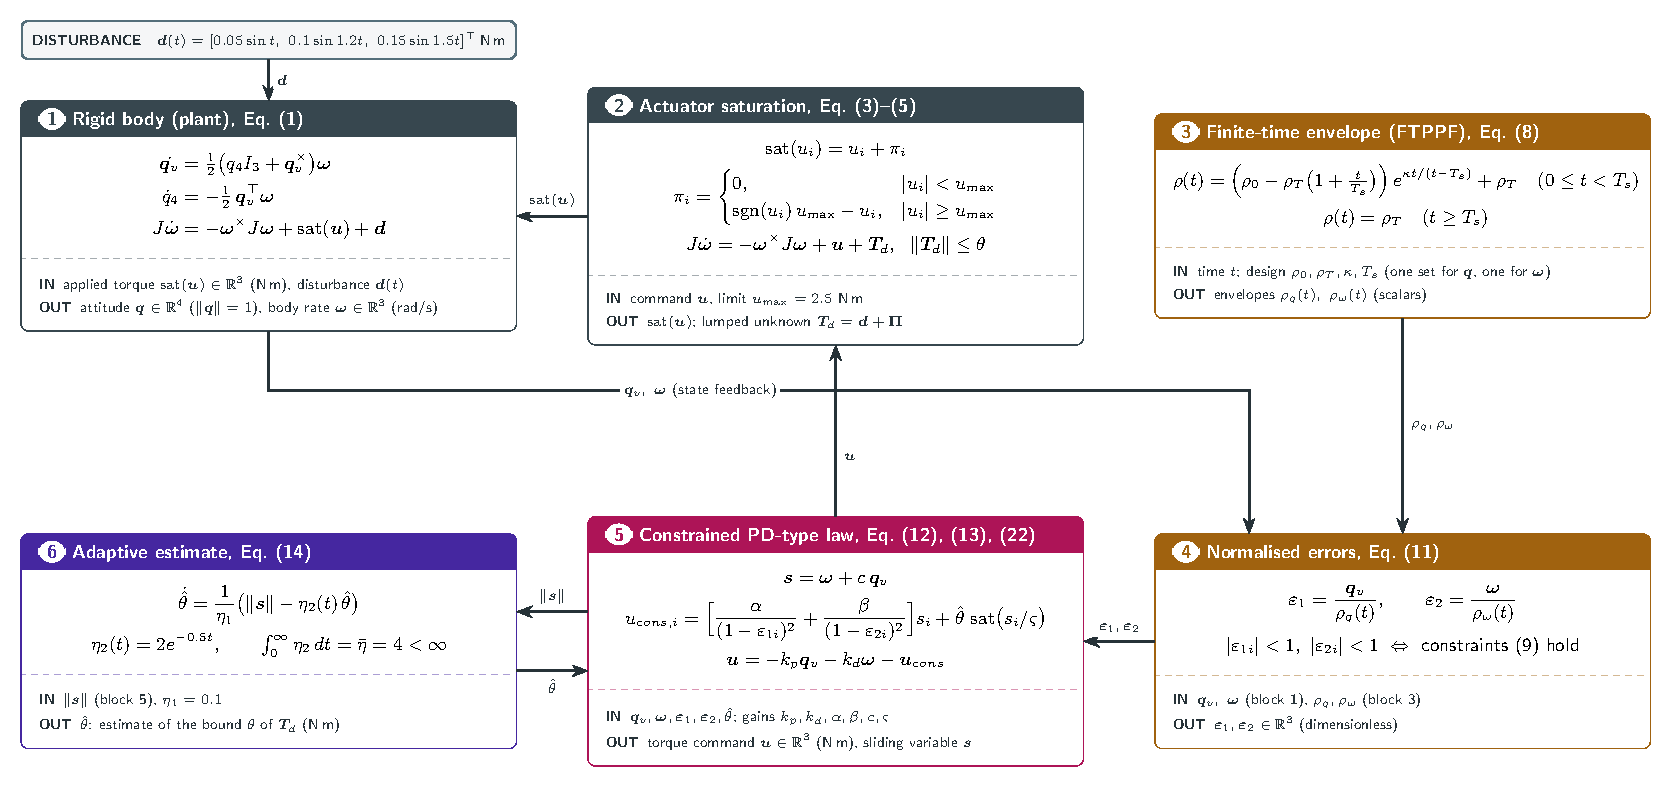
\includegraphics[width=\linewidth]{flow_paper.pdf}
\caption{Flow of the base paper (blocks 1--6). The loop is closed through the state feedback $\qv,\vw$. The disturbance
$\vd(t)$ and the saturation (block 2) are the two things the controller does not know.}
\label{fig:flowpaper}
\end{figure}

\textbf{Reading \cref{fig:flowpaper}.} The plant (block 1) produces the attitude and body rate. The envelope (block 3)
says how large they may be at time $t$; block 4 divides one by the other. The control law (block 5) uses the state,
the normalised errors and the adaptive estimate (block 6) to compute a torque. The actuators can only deliver part of it
(block 2), and that applied torque, together with the disturbance, turns the body again.

\begin{figure}[H]
\centering
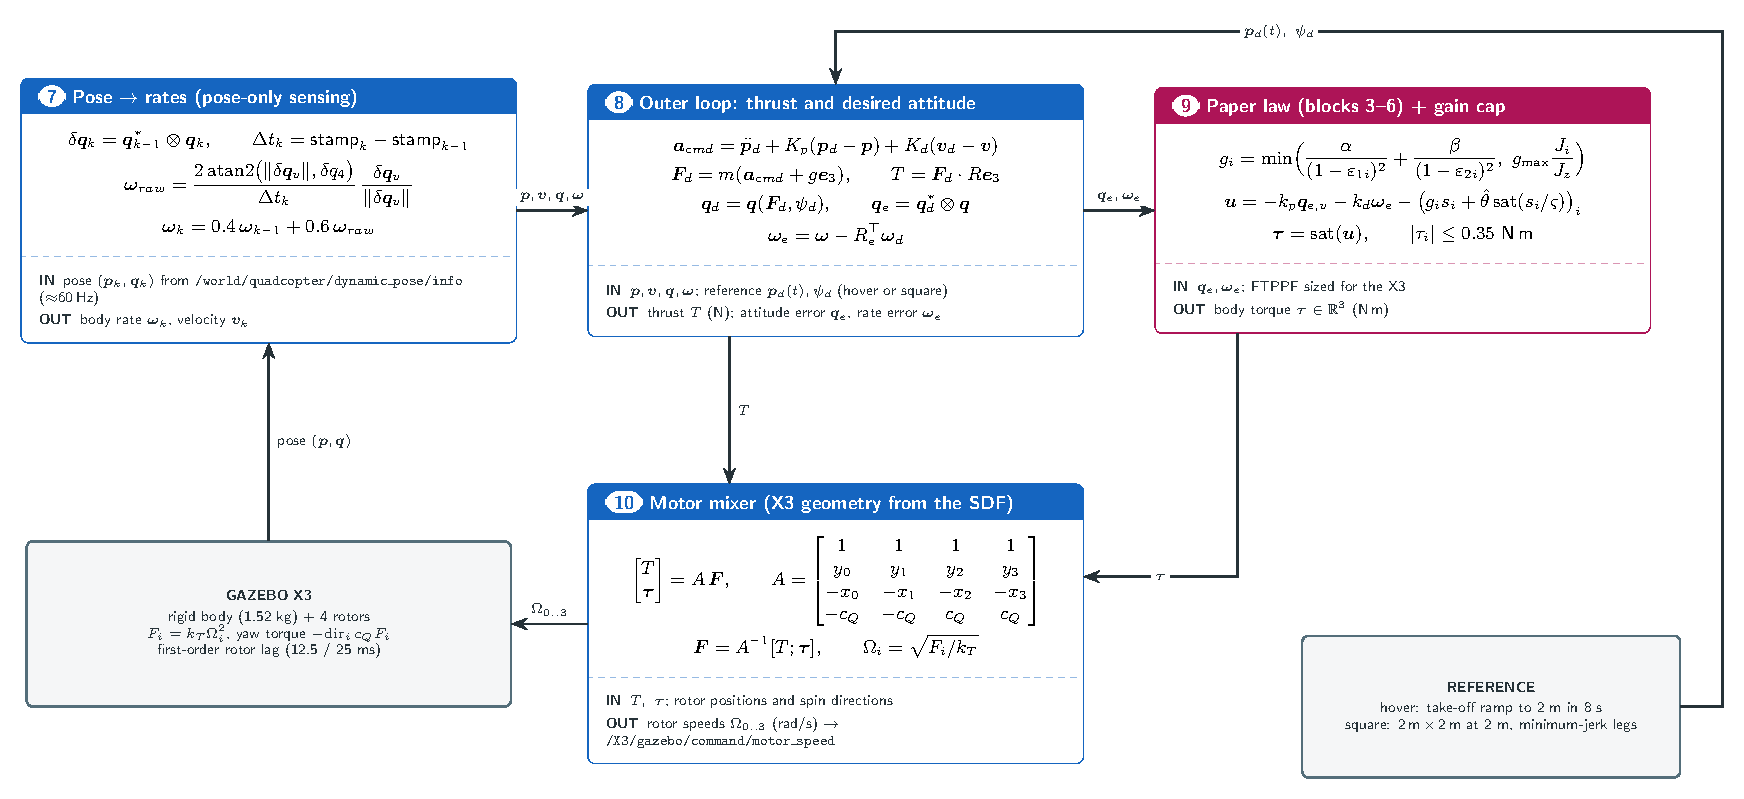
\includegraphics[width=\linewidth]{flow_x3.pdf}
\caption{Flow on the Gazebo X3 quadcopter (blocks 7--10). Blocks 3--6 of \cref{fig:flowpaper} sit inside block 9 unchanged
except for one cap on the barrier gain. Gazebo replaces blocks 1--2: it integrates the real rigid-body and rotor physics.}
\label{fig:flowx3}
\end{figure}

\textbf{Reading \cref{fig:flowx3}.} A quadcopter cannot just turn: it must also hold itself up, and it moves sideways by
tilting. So an \emph{outer} loop (block 8) decides the total thrust and the attitude the drone should have, the paper's
law (block 9) turns the body to that attitude, and the mixer (block 10) splits thrust and torque into four rotor speeds.
Gazebo only publishes the pose, so the body rate is reconstructed from two consecutive quaternions (block 7).

\begin{center}\small
\begin{tabularx}{\linewidth}{@{}c l X l@{}}
\toprule
\textbf{Block} & \textbf{Name} & \textbf{Paper equations} & \textbf{Section}\\
\midrule
1 & Rigid-body attitude dynamics & (1), (2) & \ref{sec:b1}\\
2 & Actuator saturation & (3)--(5) & \ref{sec:b2}\\
3 & Finite-time prescribed performance function & (6)--(8) & \ref{sec:b3}\\
4 & Normalised errors & (9)--(11) & \ref{sec:b4}\\
5 & Constrained PD-type control law & (12), (13), (22) & \ref{sec:b5}\\
6 & Adaptive law & (14) & \ref{sec:b6}\\
-- & Stability proof (Theorem 1) & (15)--(21) & \ref{sec:theorem}\\
7 & Body rate from the pose & -- (ours) & \ref{sec:b7}\\
8 & Outer position loop and desired attitude & -- (ours) & \ref{sec:b8}\\
9 & Paper law on a 60\,Hz loop & (12)--(14) + gain cap & \ref{sec:b9}\\
10 & X3 motor mixer & -- (ours) & \ref{sec:b10}\\
\bottomrule
\end{tabularx}
\end{center}

% =====================================================================
\section{The Paper's Model: Blocks 1--6}
\label{sec:paper}
% =====================================================================

This section follows \cref{fig:flowpaper} from the plant to the adaptive law. All numbers in the toy examples use the
paper's Part~1 initial state at $t=0$, $\vq(0)=[0.2,-0.15,-0.25,0.9354]^\top$, $\vw(0)=[0.03,0.02,-0.01]^\top$\,rad/s,
so the examples of consecutive blocks chain together: the output of one is the input of the next.

% ---------------------------------------------------------------------
\subsection{Block 1 --- How a rigid body turns}
\label{sec:b1}
% ---------------------------------------------------------------------

\begin{idea}
Two separate facts describe a turning body. \emph{Kinematics}: if it spins with rate $\vw$, its orientation changes
in a known way (this is pure geometry, no forces). \emph{Dynamics}: a torque changes the spin, and a body that spins
about two axes at once starts spinning about the third by itself (gyroscopic coupling).
\end{idea}

\begin{eqbox}{cPlant}{Equation (1): quaternion kinematics and Euler's rotational dynamics}
\begin{align}
\dot{\qv}&=\tfrac12\big(q_4I_3+\qv^{\times}\big)\vw, \qquad \dot q_4=-\tfrac12\,\qv^\top\vw \tag{1a}\label{eq:kin}\\
J\dot{\vw}&=-\vw^{\times}J\vw+\vu+\vd \tag{1b}\label{eq:dyn}
\end{align}
\end{eqbox}

\begin{dimtable}
\vq=[\qv^\top,q_4]^\top & attitude quaternion & \R^4 & --\\
\vw & body angular velocity & \R^3 & rad/s\\
J & inertia matrix & \R^{3\times3} & kg\,m$^2$\\
\vu & control torque (in block 2 replaced by $\sat(\vu)$) & \R^3 & N\,m\\
\vd & disturbance torque & \R^3 & N\,m\\
I_3 & $3\times3$ identity & \R^{3\times3} & --\\
\end{dimtable}

\subsubsection*{Where (1a) comes from}
Rotating first by $\vq$ and then by a tiny extra rotation $\vw\,dt$ (measured in the body frame) is the quaternion
product $\vq(t+dt)=\vq(t)\otimes[\tfrac12\vw\,dt;\ 1]$, because by \eqref{eq:quat} a small angle $\phi$ about $\bm n$ is
$[\tfrac{\phi}{2}\bm n;\ 1]$. Hence $\dot\vq=\tfrac12\,\vq\otimes[\vw;0]$. Writing out the Hamilton product
$[\bm a;a_4]\otimes[\bm b;b_4]=[a_4\bm b+b_4\bm a+\bm a\times\bm b;\ a_4b_4-\bm a^\top\bm b]$ with $\bm a=\qv$, $a_4=q_4$,
$\bm b=\vw$, $b_4=0$ gives
\[
\dot\vq=\tfrac12\begin{bmatrix}q_4\vw+\qv\times\vw\\ -\qv^\top\vw\end{bmatrix}
=\begin{bmatrix}\tfrac12(q_4I_3+\qv^\times)\vw\\ -\tfrac12\qv^\top\vw\end{bmatrix},
\]
which is (1a). It keeps $\|\vq\|=1$: $\tfrac{d}{dt}\|\vq\|^2=2\qv^\top\dot\qv+2q_4\dot q_4=\qv^\top\qv^\times\vw=0$, since
$\qv^\top(\qv\times\vw)=0$. (A numerical integrator does not keep it exactly, so every simulation re-normalises $\vq$ after
each step.)

\subsubsection*{Where (1b) comes from}
The angular momentum in the body frame is $\bm h=J\vw$. In the inertial frame Newton's law for rotation is
$\tfrac{d}{dt}\bm h_{\mathcal F_i}=$ torque. The body frame itself turns with $\vw$, and the derivative of any vector
seen from a turning frame picks up the term $\vw\times(\cdot)$:
\[
\tfrac{d}{dt}\bm h\big|_{\mathcal F_i}=J\dot\vw+\vw\times J\vw=\vu+\vd
\quad\Longrightarrow\quad J\dot\vw=-\vw^\times J\vw+\vu+\vd .
\]
The term $-\vw^\times J\vw$ is the gyroscopic coupling. It does no work: $\vw^\top(\vw^\times J\vw)=0$ by the
skew-symmetry of \eqref{eq:skew}. This is used in the proof of Theorem~1.

\begin{toybox}[one evaluation of Eq. (1) at the Part-1 initial state]
$q_4\vw=0.9354\,[0.03,0.02,-0.01]=[0.02806,\,0.01871,\,-0.00935]$ and
$\qv\times\vw=[0.0065,\,-0.0055,\,0.0085]$. Their sum times $\tfrac12$:
\[
\dot\qv=[0.01728,\ 0.00660,\ -0.00043]^\top\ \text{s}^{-1},\qquad \dot q_4=-\tfrac12\qv^\top\vw=-0.00275\ \text{s}^{-1}.
\]
Dynamics with the torque the controller will apply at $t=0$ (block~5 shows it saturates at $[-2.5,2.5,2.5]$\,N\,m) and
$\vd(0)=0$: $J\vw=[0.615,\,0.362,\,-0.095]$, $\vw\times J\vw=[0.00172,\,-0.0033,\,-0.00144]$, and
\[
\dot\vw=J^{-1}\big(-\vw\times J\vw+\sat(\vu)\big)=[-0.141,\ 0.144,\ 0.162]^\top\ \text{rad/s}^2 .
\]
Even at full torque the heavy spacecraft accelerates by only $\approx0.15$\,rad/s$^2$. Remember this number: it
decides which envelopes are feasible (complete documentation, Monte-Carlo study C).
\end{toybox}

\begin{projbox}
\code{paper\_reproduction.py}, function \code{rhs()}, evaluates (1a)--(1b) for a whole batch of simulations at once and
is integrated with RK4 at $\Delta t=1$\,ms; MATLAB \code{step6\_spacecraft\_closed\_loop.m} contains an independent
re-implementation. On the X3 we do \emph{not} integrate (1): Gazebo does, for the real quadcopter (\cref{sec:x3}).
\end{projbox}

% ---------------------------------------------------------------------
\subsection{Block 2 --- What the actuators can really do}
\label{sec:b2}
% ---------------------------------------------------------------------

\begin{idea}
Reaction wheels or rotors have a maximum torque. Whatever the controller asks for beyond it is simply not
delivered. The paper does not ignore this: it treats the missing torque as one more unknown disturbance.
\end{idea}

\begin{eqbox}{cPlant}{Equations (3)--(5): saturation and the lumped unknown torque}
\begin{align}
\sat(u_i)&=u_i+\pi_i,\qquad
\pi_i=\begin{cases}0,& |u_i|<\umax\\ \sgn(u_i)\,\umax-u_i,& |u_i|\ge\umax\end{cases}\tag{3--4}\\
J\dot\vw&=-\vw^\times J\vw+\vu+\bm T_d,\qquad \bm T_d=\vd+\bm\Pi,\quad \|\bm T_d\|\le\theta \tag{5}\label{eq:lumped}
\end{align}
\end{eqbox}

\begin{dimtable}
\umax & torque limit of each axis & \R & N\,m\\
\pi_i & torque lost on axis $i$ & \R & N\,m\\
\bm T_d & disturbance plus lost torque & \R^3 & N\,m\\
\theta & an (unknown) upper bound of $\|\bm T_d\|$ & \R & N\,m\\
\end{dimtable}

\subsubsection*{Derivation}
(3)--(4) is just $\sat(u_i)=\sgn(u_i)\min(|u_i|,\umax)$ written as ``command plus error''. Putting $\sat(\vu)=\vu+\bm\Pi$
into (1b) and collecting everything the controller does not know into $\bm T_d$ gives (5). The trick is that now the
plant looks as if it received the \emph{commanded} torque, plus one bounded unknown. The adaptive law (block~6) will
estimate a bound for it. $\theta$ is bounded because $\vd$ is bounded and because $\vu$ stays bounded (all its terms are
bounded while the state is inside the envelope).

\begin{toybox}[the torque lost at $t=0$]
Block 5 will compute $\vu(0)=[-10.537,\ 5.710,\ 10.414]^\top$\,N\,m. With $\umax=2.5$ every axis saturates:
$\sat(\vu)=[-2.5,\ 2.5,\ 2.5]$ and $\bm\Pi=\sat(\vu)-\vu=[8.037,\ -3.210,\ -7.914]$\,N\,m. At the very start the
``unknown'' torque is dominated by saturation, not by the disturbance (whose size is at most 0.187\,N\,m).
\end{toybox}

\begin{projbox}
\code{sat\_vec()} in \code{paper\_reproduction.py} clips each axis at 2.5\,N\,m; on the X3 the torque is clipped at
0.35\,N\,m and, in addition, the mixer must keep every rotor between 0 and 800\,rad/s (block 10).
\end{projbox}

% ---------------------------------------------------------------------
\subsection{Block 3 --- The finite-time envelope (FTPPF)}
\label{sec:b3}
% ---------------------------------------------------------------------

\begin{idea}
Draw a tube around zero that starts wide and narrows with time. If the state never touches the walls of the tube,
then automatically: its overshoot is smaller than the initial width, it is at least as fast as the walls close, and
its final error is smaller than the final width. The paper's new tube reaches its final width \emph{exactly} at a chosen
time $T_s$ and then stays constant, instead of only approaching it.
\end{idea}

\begin{eqbox}{cEnv}{Equations (6)--(8): performance constraint and finite-time prescribed performance function}
\begin{align}
-\rho_q(t)&<q_i(t)<\rho_q(t),\qquad -\rho_\omega(t)<\omega_i(t)<\rho_\omega(t),\qquad i=1,2,3 \tag{6, 9}\label{eq:constraint}\\
\rho(t)&=\begin{cases}\Big(\rho_0-\rho_T\big(1+\tfrac{t}{T_s}\big)\Big)\exp\!\Big(\dfrac{\kappa\,t}{t-T_s}\Big)+\rho_T,&0\le t<T_s\\[4pt]
\rho_T,& t\ge T_s\end{cases}\tag{8}\label{eq:ftppf}
\end{align}
For comparison, the classical exponential PPF is $\rho(t)=(\rho_0-\rho_\infty)e^{-\kappa t}+\rho_\infty$ (Eq.~7).
\end{eqbox}

\begin{dimtable}
\rho_0 & initial width: the largest allowed $|q_i|$ (or $|\omega_i|$) & \R & --, rad/s\\
\rho_T & final width: the guaranteed accuracy after $T_s$ & \R & --, rad/s\\
T_s & settling time of the envelope & \R & s\\
\kappa & shape: how early the envelope starts to close & \R & --\\
\end{dimtable}

\subsubsection*{Checking the three properties}
\begin{enumerate}[leftmargin=*]
  \item \emph{Start.} At $t=0$ the exponent is $0$, so $\rho(0)=(\rho_0-\rho_T)\cdot1+\rho_T=\rho_0$.
  \item \emph{Arrival exactly at $T_s$.} For $t\to T_s^-$ the denominator $t-T_s\to0^-$ while the numerator $\kappa t>0$,
        so the exponent $\to-\infty$ and $\exp(\cdot)\to0$. The bracket stays finite ($\to\rho_0-2\rho_T$), hence
        $\rho\to\rho_T$, and the second line continues it. So $\rho$ is continuous and equals $\rho_T$ from $T_s$ on.
        The exponential PPF instead only gets there as $t\to\infty$.
  \item \emph{It never increases and never dips below $\rho_T$.} If $\rho_0>2\rho_T$ (true for every envelope we use),
        the bracket $b(t)=\rho_0-\rho_T(1+t/T_s)$ is positive on $[0,T_s)$, so $\rho>\rho_T$ there. Differentiating,
        \[
        \dot\rho(t)=\Big(-\frac{\rho_T}{T_s}-b(t)\,\frac{\kappa T_s}{(t-T_s)^2}\Big)\exp\!\Big(\frac{\kappa t}{t-T_s}\Big)<0,
        \]
        because $\tfrac{d}{dt}\tfrac{\kappa t}{t-T_s}=-\tfrac{\kappa T_s}{(t-T_s)^2}$. Both terms are negative.
\end{enumerate}

\begin{toybox}[$\rho_q(2)$ with the paper's attitude envelope, $T_s=15$\,s]
$\rho_0=0.3$, $\rho_T=0.008$, $\kappa=2.5$:
\[
b(2)=0.3-0.008\Big(1+\tfrac{2}{15}\Big)=0.290933,\qquad \exp\!\Big(\tfrac{2.5\cdot2}{2-15}\Big)=e^{-0.38462}=0.680712,
\]
\[
\rho_q(2)=0.290933\times0.680712+0.008=0.206042 .
\]
The same for the rate envelope ($\rho_0=0.4$, $\rho_T=0.005$): $\rho_\omega(2)=0.394333\times0.680712+0.005=0.273428$\,rad/s.
Values along the way (from the same formula): $\rho_q=0.300,\ 0.252,\ 0.206,\ 0.091,\ 0.0245,\ 0.0099,\ 0.0080$ at
$t=0,1,2,5,8,10,12$\,s. With $T_s=10$\,s instead, $\rho_q(5)=0.0316$: a shorter $T_s$ closes the tube faster.
\end{toybox}

\begin{toybox}[finite time versus exponential, $T_s=8$\,s]
Exponential PPF with $\kappa=0.5$ at $t=8$\,s: $(0.3-0.008)e^{-4}+0.008=0.01335$, still $1.67\times\rho_T$. The FTPPF is
exactly $0.008$ at $8$\,s.
\end{toybox}

\begin{codebox}
\textbf{MATLAB:} \code{toy\_model/step1\_ftppf.m}. Part A prints the three numbers $0.290933$, $0.680712$, $0.206042$;
Part B checks $\rho(0)=\rho_0$, $\rho(T_s)=\rho_T$, monotonicity, and plots the effect of $T_s$ and $\kappa$.
Library function: \code{toy\_model/lib/ftppf.m}.
\end{codebox}

\begin{projbox}
\code{ftppf()} in \code{paper\_reproduction.py} (vectorised) and in \code{x3\_sim/controllers.py} (scalar, with a guard
that returns $\rho_T$ once the exponent is below $-50$ to avoid underflow). The paper's values are used for the
spacecraft; on the X3 the envelope is re-sized to $\rho_q:0.30\to0.02$, $\rho_\omega:2.5\to0.05$\,rad/s, $\kappa=2$,
$T_s=10$\,s (\cref{sec:b9}).
\end{projbox}

% ---------------------------------------------------------------------
\subsection{Block 4 --- Normalised errors}
\label{sec:b4}
% ---------------------------------------------------------------------

\begin{idea}
Instead of transforming the error through a complicated function (classical PPC), simply divide it by the current
half-width of the tube. The result says ``what fraction of the allowed room is used''. Inside the tube means
$|\varepsilon|<1$.
\end{idea}

\begin{eqbox}{cEnv}{Equation (11): the simple error transformation}
\begin{equation}
\veps_1=\frac{\qv(t)}{\rho_q(t)},\qquad \veps_2=\frac{\vw(t)}{\rho_\omega(t)},\qquad
\text{(9) holds}\iff |\varepsilon_{1i}(t)|<1\ \text{and}\ |\varepsilon_{2i}(t)|<1\ \ \forall i \tag{11}\label{eq:eps}
\end{equation}
\end{eqbox}

\begin{dimtable}
\veps_1=[\varepsilon_{11},\varepsilon_{12},\varepsilon_{13}]^\top & attitude error as a fraction of $\rho_q$ & \R^3 & --\\
\veps_2=[\varepsilon_{21},\varepsilon_{22},\varepsilon_{23}]^\top & rate error as a fraction of $\rho_\omega$ & \R^3 & --\\
\end{dimtable}

\subsubsection*{Why this is enough}
$\rho_q,\rho_\omega>0$ always, so dividing by them does not change signs and $|q_i|<\rho_q\iff|q_i/\rho_q|<1$. Nothing has
to be differentiated: classical PPC would need $\partial S^{-1}/\partial(\cdot)$ and $\dot\rho$ inside the controller. A
necessary condition is that the state \emph{starts} inside: $|q_i(0)|<\rho_{q0}$ and $|\omega_i(0)|<\rho_{\omega0}$
(paper Remark~7).

\begin{toybox}[Part-1 state at $t=0$ ($\rho_q=0.3$, $\rho_\omega=0.4$)]
\[
\veps_1=\frac{[0.2,\ -0.15,\ -0.25]}{0.3}=[0.6667,\ -0.5,\ -0.8333],
\]
\[
\veps_2=\frac{[0.03,\ 0.02,\ -0.01]}{0.4}=[0.075,\ 0.05,\ -0.025].
\]
All six are below 1 in magnitude: the start is admissible. Axis 3 uses 83\,\% of its attitude room.

Part-2 state with the paper's $\rho_{q0}=0.3$: $\varepsilon_{11}=0.3/0.3=1$ exactly. The constraint is violated at $t=0$
and $(1-\varepsilon_{11})^{-2}=1/0$. This is why we use $\rho_{q0}=0.36$ for Part~2 (\cref{warn:part2}); then
$\veps_1(0)=[0.833,\,-0.556,\,-0.833]$.
\end{toybox}

\begin{codebox}
\textbf{MATLAB:} \code{toy\_model/step2\_normalised\_error.m}, Part A, prints $\veps_1$, $\veps_2$ and the gains of block~5.
\end{codebox}

% ---------------------------------------------------------------------
\subsection{Block 5 --- The constrained PD-type control law}
\label{sec:b5}
% ---------------------------------------------------------------------

\begin{idea}
A spring and a damper: the PD part pulls the attitude error to zero ($-k_p\qv$, the spring) and brakes the rotation
($-k_d\vw$, the damper). On top of that, a second, \emph{variable} damper acts on the combination $\vs=\vw+c\qv$: its
strength is small in the middle of the tube and becomes huge near the wall. Finally $\that\,\sat(\vs/\varsigma)$ adds a
push of size $\that$ against the unknown torque.
\end{idea}

\begin{eqbox}{cCtrl}{Equations (12), (13) and (22): the controller}
\begin{align}
\vu&=-k_p\qv-k_d\vw-\vu_{cons} \tag{12}\label{eq:law}\\
\vu_{cons}&=\Big[\alpha(1-\veps_1)^{-2}+\beta(1-\veps_2)^{-2}\Big]\vs+\that\,\sgn(\vs),\qquad \vs=\vw+c\,\qv \tag{13}\label{eq:ucons}\\
u_{cons,i}&=\Big[\frac{\alpha}{(1-\varepsilon_{1i})^{2}}+\frac{\beta}{(1-\varepsilon_{2i})^{2}}\Big]s_i+\that\,\sat\!\Big(\frac{s_i}{\varsigma}\Big)
\quad\text{(Remark 5, chattering-free form)} \tag{22}\label{eq:ucons22}
\end{align}
\end{eqbox}

\begin{dimtable}
\vs & sliding variable, a ``target'' rate $-c\qv$ compared with $\vw$ & \R^3 & rad/s\\
g_i=\frac{\alpha}{(1-\varepsilon_{1i})^2}+\frac{\beta}{(1-\varepsilon_{2i})^2} & barrier gain of axis $i$ & \R & N\,m\,s\\
k_p,\ k_d & PD gains (40, 20) & \R & N\,m, N\,m\,s\\
\alpha,\ \beta & barrier weights (1.5, 1.2) & \R & N\,m\,s\\
c & weight of $\qv$ in $\vs$ (0.5) & \R & s$^{-1}$\\
\varsigma & boundary-layer width (0.02) & \R & rad/s\\
\end{dimtable}

\subsubsection*{How the barrier term keeps the state inside}
\begin{enumerate}[leftmargin=*]
  \item In the middle of the tube ($\veps\approx0$) the gain is $g_i\approx\alpha+\beta=2.7$, small next to $k_d=20$: the
        controller behaves like plain PD.
  \item As the state approaches the wall, $\varepsilon\to1$ and $(1-\varepsilon)^{-2}\to\infty$. The term $-g_is_i$ then
        dominates. Because $\vs=\vw+c\qv$, a large negative feedback on $s_i$ drives $\omega_i$ towards $-cq_i$, i.e.\ it makes
        the body rotate \emph{back towards zero} and caps its speed. This is Remark~2/Remark~7 of the paper.
  \item $\vs$ is the natural variable: when $\vs=0$ we have $\vw=-c\qv$, which by (1a) makes $\qv$ decay
        ($\tfrac{d}{dt}\|\qv\|^2=2\qv^\top\dot\qv=q_4\qv^\top\vw=-c\,q_4\|\qv\|^2<0$ for $q_4>0$). Pushing $\vs$ to zero
        therefore also pushes the attitude error to zero.
\end{enumerate}

\begin{warn}[A detail the paper leaves open: one-sided or two-sided barrier?]
Written literally, $(1-\varepsilon_{1i})^{-2}$ grows only as $\varepsilon_{1i}\to+1$. As $\varepsilon_{1i}\to-1$ it tends to
$1/4$. So the paper's barrier protects the upper wall of the tube much more strongly than the lower wall. A symmetric
alternative is $\alpha(1-\varepsilon_{1i}^2)^{-2}$, which grows at both walls; our first browser and Gazebo code used it.
We treat the \textbf{paper form as the reference} and report the symmetric form as a clearly labelled variant
(``symmetric barrier'') everywhere. Both are compared in the complete documentation.
\end{warn}

\begin{toybox}[the torque at $t=0$ for the Part-1 state, $\that(0)=0$]
Sliding variable: $\vs=\vw+0.5\,\qv=[0.03+0.1,\ 0.02-0.075,\ -0.01-0.125]=[0.13,\ -0.055,\ -0.135]$\,rad/s.

PD part: $-40\qv-20\vw=[-8+(-0.6),\ 6-0.4,\ 10+0.2]=[-8.6,\ 5.6,\ 10.2]$\,N\,m.

Barrier gains (paper form) with $\veps_1,\veps_2$ from block 4:
\[
g_1=\frac{1.5}{(1-0.6667)^2}+\frac{1.2}{(1-0.075)^2}=13.500+1.403=14.903,\quad g_2=1.996,\quad g_3=1.588 .
\]
$\vu_{cons}=g\odot\vs=[1.937,\ -0.110,\ -0.214]$, and
\[
\vu=[-8.6,\ 5.6,\ 10.2]-[1.937,\ -0.110,\ -0.214]=[-10.537,\ 5.710,\ 10.414]\ \text{N\,m}.
\]
Every axis exceeds 2.5\,N\,m, so $\sat(\vu)=[-2.5,\,2.5,\,2.5]$ (block 2). Note the one-sided effect: axis 3 is
\emph{closest} to its wall ($|\varepsilon_{13}|=0.833$) but gets the \emph{smallest} gain, because $\varepsilon_{13}<0$. With
the symmetric form the gains would be $[6.07,\ 3.87,\ 17.27]$ and $\vu=[-9.39,\ 5.81,\ 12.53]$.
\end{toybox}

\begin{codebox}
\textbf{MATLAB:} \code{step2\_normalised\_error.m} prints the gains $g$ of both forms and plots them over $\varepsilon$;
\code{step3\_control\_law.m} prints $\vs$, $\vu_{PD}$, $\vu_{cons}$, $\vu$ and $\sat(\vu)$ for the three controllers.
Library function: \code{toy\_model/lib/control\_law.m}.
\end{codebox}

\begin{projbox}
\code{control()} in \code{paper\_reproduction.py} implements (12) and (22) with \code{mode = "constrained"} (paper form),
\code{"symmetric"} or \code{"pd"} ($\vu_{cons}=0$). The value of $\varepsilon$ fed to the barrier is limited to $0.999$; this
guard is never active while the state is inside the envelope and only prevents a division by zero if it ever leaves.
\pyfile{117}{140}{\repro}{paper\_reproduction.py --- control(): Eq. (11), (12), (22)}
\end{projbox}

% ---------------------------------------------------------------------
\subsection{Block 6 --- The adaptive estimate}
\label{sec:b6}
% ---------------------------------------------------------------------

\begin{idea}
The controller does not know how large the disturbance plus the lost torque is. So it learns a number $\that$: it
grows while the sliding variable is not zero (``something is still pushing me away'') and is slowly pulled back by a
leakage term. $\that$ then sets the size of the push $\that\,\sat(\vs/\varsigma)$ in block 5.
\end{idea}

\begin{eqbox}{cAdapt}{Equation (14): adaptive law}
\begin{equation}
\dot{\that}=\frac{1}{\eta_1}\Big(\|\vs\|-\eta_2(t)\,\that\Big),\qquad \eta_1>0,\qquad
\int_0^\infty\eta_2(\tau)\,d\tau=\bar\eta<\infty \tag{14}\label{eq:adapt}
\end{equation}
Paper choice: $\eta_1=0.1$, $\eta_2(t)=2e^{-0.5t}$ (so $\bar\eta=2/0.5=4$), $\that(0)=0$.
\end{eqbox}

\subsubsection*{Reading the law}
Without leakage ($\eta_2=0$), $\that$ is the time integral of $\|\vs\|/\eta_1$: it keeps growing as long as $\vs\ne0$. The
leakage $-\eta_2\that$ pulls it down. The paper requires $\eta_2$ to have a \emph{finite} integral, which means the leakage
dies out with time; this is what makes the extra term in the Lyapunov inequality bounded (\cref{sec:theorem}).

\begin{toybox}[one Euler step, $\Delta t=1$\,ms, from $\that=0$]
$\|\vs(0)\|=\sqrt{0.13^2+0.055^2+0.135^2}=0.19532$. Then
$\that(1\,\text{ms})=0+0.001\times(0.19532-2\cdot0)/0.1=0.0019532$\,N\,m.
\end{toybox}

\begin{warn}[What the leakage that dies out means in practice]
With the chattering-free form (22) the sliding variable does not become exactly zero: inside the boundary layer
$\that\,\sat(s_i/\varsigma)$ is smaller than $\that$, so a small residual $\|\vs\|$ remains while the disturbance acts. Because
$\eta_2\to0$, nothing then stops $\that$ from creeping upwards slowly (``parameter drift''). We observe exactly this
in the reproduction: $\that$ is still rising at $t=20$\,s ($\approx0.43$), although the state has long converged. It is
harmless over the paper's horizon, but on the X3, which runs for 180\,s, we keep $\eta_2\ge0.2$ and $\that\le0.1$\,N\,m.
\code{step4\_adaptive\_law.m} shows the three cases side by side.
\end{warn}

\begin{projbox}
In \code{paper\_reproduction.py} the law is integrated with explicit Euler at 1\,ms after each RK4 step, with the
projection $\that\ge0$ (an estimate of a bound cannot be negative):
\pyfile{190}{192}{\repro}{paper\_reproduction.py --- adaptive law, Eq. (14)}
\end{projbox}

% ---------------------------------------------------------------------
\subsection{Theorem 1 --- Why the closed loop converges}
\label{sec:theorem}
% ---------------------------------------------------------------------

\begin{eqbox}{cCtrl}{Theorem 1 of the paper and its Lyapunov function (15)}
For the system (5) under the control (12)--(14), $\qv(t)\to0$ and $\vw(t)\to0$ as $t\to\infty$. Proof candidate:
\begin{equation}
V=(k_p+ck_d)\big(\qv^\top\qv+(1-q_4)^2\big)+\tfrac12\vw^\top J\vw+c\,\qv^\top J\vw+\tfrac{\eta_1}{2}\,\ttil^{\,2},
\qquad \ttil=\theta-\that \tag{15}\label{eq:V}
\end{equation}
\end{eqbox}

\subsubsection*{The argument in four steps}
\begin{enumerate}[leftmargin=*]
  \item \textbf{$V$ is a valid ``energy''.} Using $|c\,\qv^\top J\vw|\le c\,\lambda_{\max}(J)\|\qv\|\|\vw\|$ and
        $\tfrac12\vw^\top J\vw\ge\tfrac12\lambda_{\min}(J)\|\vw\|^2$, $V\ge\tfrac12\bm x^\top P\bm x$ with
        $\bm x=[\|\qv\|,\ \|\vw\|,\ |\ttil|]^\top$ and
        \[
        P=\begin{bmatrix}2(k_p+ck_d)&-c\lambda_{\max}(J)&0\\-c\lambda_{\max}(J)&\lambda_{\min}(J)&0\\0&0&\eta_1\end{bmatrix}.
        \]
        $P\succ0$ needs $2(k_p+ck_d)\lambda_{\min}(J)>(c\lambda_{\max}(J))^2$.
  \item \textbf{Differentiate along the motion.} Using (1a), (5), (12), the skew-symmetry of $\vw^\times$ and $\dot\ttil=-\dot\that$,
        the paper obtains (Eq.~17)
        \[
        \dot V=-ck_p\|\qv\|^2-k_d\|\vw\|^2+\vs^\top\bm T_d+\tfrac c2\big(q_4\vw+\vw^\times\qv\big)^\top J\vw
        -\vs^\top\big[\cdots\big]\vs-\|\vs\|\that-\ttil\big(\|\vs\|-\eta_2\that\big).
        \]
        The barrier term $-\vs^\top[\cdots]\vs$ is $\le0$ because its gain is positive (Remark~2) and can be dropped.
        Since $\vs^\top\bm T_d\le\|\vs\|\theta$, the terms with $\|\vs\|$ combine to $\|\vs\|(\theta-\that-\ttil)=0$.
  \item \textbf{Bound the leakage term} with $\ttil\that\le-\tfrac{2\sigma-1}{2\sigma}\ttil^2+\tfrac{\sigma}{2}\theta^2$ (Eq.~18),
        which gives $\dot V\le-\bm x^\top Q\bm x+\tfrac{\eta_2\sigma}{2}\theta^2$ with
        $Q=\diag\big(ck_p,\ k_d-c\lambda_{\max}(J),\ \eta_2\tfrac{2\sigma-1}{2\sigma}\big)$ (Eq.~19). $Q\succ0$ needs
        $c<k_d/\lambda_{\max}(J)$ and $\sigma>\tfrac12$.
  \item \textbf{Integrate and use Barbalat.} $V(t)\le V(0)-\lambda_{\min}(Q)\int_0^t\|\bm x\|^2+\tfrac{\sigma}{2}\theta^2\bar\eta$,
        so $V$ stays bounded, $\qv,\vw\in\mathcal L_2$, their derivatives are bounded, and Barbalat's lemma gives
        $\qv\to0$, $\vw\to0$.
\end{enumerate}

\begin{toybox}[the two conditions on $c$ with the paper's numbers]
$\lambda_{\min}(J)=14.27$, $\lambda_{\max}(J)=20.74$, $k_p=40$, $k_d=20$, $c=0.5$:
\[
Q:\quad k_d-c\lambda_{\max}=20-10.37=9.63>0\qquad(\text{i.e. } c<20/20.74=0.964),
\]
\[
P:\quad 2(40+10)\cdot14.27=1427>(0.5\cdot20.74)^2=107.5 .
\]
Both hold, so our unstated choice $c=0.5$ satisfies the theorem.
\end{toybox}

\begin{warn}[Three things a careful reader notices in the proof]
\begin{enumerate}[leftmargin=*]
  \item \textbf{What is proved.} Theorem 1 proves \emph{convergence to the origin}. It does not separately prove that
        $|\varepsilon_{li}(t)|<1$ is preserved for all $t$ (that the state never leaves the tube); the paper supports that
        with Remarks 2 and 7 and with simulations. We therefore phrase our own claims as ``constraint satisfaction
        observed in simulation'' and measure it.
  \item \textbf{Printing details of Eq.~(15).} The paper prints $(1-q_0^2)$ and $\tfrac{1}{\eta_1}\ttil^2$. With
        $(1-q_0)^2$ (the form of the cited reference [42]) and the weight $\tfrac{\eta_1}{2}$, differentiating gives exactly
        the terms of Eq.~(17); we write (15) in that consistent form. The conclusions do not change.
  \item \textbf{The proof uses $\sgn(\vs)$.} With the boundary layer (22) the cancellation in step 2 is exact only for
        $|s_i|\ge\varsigma$; inside the layer a residual of order $\varsigma$ remains. The practical guarantee is convergence to
        a small neighbourhood of zero, and $\that$ can drift (block~6). This matches what all our simulations show: the
        final $\|\vw\|$ is about $0.004$\,rad/s, not exactly zero.
\end{enumerate}
\end{warn}

\begin{projbox}
\code{lyapunov()} in \code{paper\_reproduction.py} evaluates the state part of (15) along the Part~2 trajectory
(figure \code{fig08\_theta\_hat\_and\_lyapunov.png}). The $\ttil$ term cannot be plotted, because the true bound $\theta$ of
$\bm T_d$ is unknown.
\end{projbox}

% =====================================================================
\section{The Quadcopter Model: Blocks 7--10}
\label{sec:x3}
% =====================================================================

The paper controls a body that can produce torque about every axis directly and does not need to hold itself up. A
quadcopter is different in three ways: (i) its four rotors produce one thrust along the body $z$-axis plus three torques,
so attitude and position are coupled (it moves sideways by tilting); (ii) Gazebo publishes only the \emph{pose}, not the
angular velocity; (iii) the controller runs as a sampled loop at the pose rate ($\approx$60\,Hz) with a transport delay.
Blocks 7--10 are what we added so that blocks 3--6 can be used unchanged on the X3. First, the physics that Gazebo
integrates (and that our software-in-the-loop surrogate \code{x3\_sim/x3\_model.py} reproduces).

\begin{eqbox}{cPlant}{The X3 quadcopter as Gazebo simulates it}
\begin{align}
m\ddot{\vp}&=R\begin{bmatrix}0\\0\\\sum_iF_i\end{bmatrix}-mg\,\bm e_3-\Big(\sum_i|\Omega_i|\Big)c_D\,\vv_\perp,\qquad F_i=k_T\Omega_i^2 \tag{X1}\label{eq:x3trans}\\
\dot\vq&=\tfrac12\,\vq\otimes[\vw;0],\qquad J\dot\vw=-\vw^\times J\vw+\vtau,\qquad
\vtau=\sum_i\Big(\vr_i\times F_i\bm e_3-\mathrm{dir}_i\,c_QF_i\,\bm e_3\Big) \tag{X2}\label{eq:x3rot}\\
\dot\Omega_i&=\frac{\Omega_{i,cmd}-\Omega_i}{\tau_{\uparrow/\downarrow}},\qquad \tau_\uparrow=12.5\ \text{ms},\ \tau_\downarrow=25\ \text{ms},\qquad 0\le\Omega_{i,cmd}\le800\ \text{rad/s} \tag{X3}\label{eq:x3rotor}
\end{align}
\end{eqbox}

\begin{dimtable}
\vp,\ \vv & position and velocity of the CoM (world) & \R^3 & m, m/s\\
R & rotation matrix of $\vq$ (body $\to$ world) & \R^{3\times3} & --\\
F_i,\ \Omega_i & thrust and speed of rotor $i$ & \R & N, rad/s\\
\vr_i & position of rotor $i$ in the body frame & \R^3 & m\\
\mathrm{dir}_i & $+1$ counter-clockwise, $-1$ clockwise rotor & \R & --\\
c_D & rotor drag coefficient ($8.06\times10^{-5}$) & \R & N\,s$^2$/(m\,rad)\\
\vv_\perp & velocity component perpendicular to the rotor axis & \R^3 & m/s\\
\end{dimtable}

(X2) is exactly the paper's Eq.~(1) with $\vu+\vd$ replaced by the torque of the rotors: the attitude part of the X3
\emph{is} the paper's plant, with a 250 times smaller inertia. (X1) is what the paper does not have.

% ---------------------------------------------------------------------
\subsection{Block 7 --- Body rate from two poses}
\label{sec:b7}
% ---------------------------------------------------------------------

\begin{idea}
If we know the orientation now and one sample ago, the small rotation between them, divided by the time between
them, is the body rate. The small rotation must be computed \emph{in the body frame} ($\vq_{k-1}^*\otimes\vq_k$), not by
subtracting quaternion components.
\end{idea}

\begin{eqbox}{cX3}{Block 7: exact body rate from consecutive quaternions}
\begin{equation}
\delta\vq_k=\vq_{k-1}^{*}\otimes\vq_k,\qquad
\vw_{raw}=\frac{2\,\mathrm{atan2}\big(\|\delta\vq_v\|,\,\delta q_4\big)}{\Delta t_k}\;\frac{\delta\vq_v}{\|\delta\vq_v\|},\qquad
\vw_k=0.4\,\vw_{k-1}+0.6\,\vw_{raw} \tag{B7}\label{eq:b7}
\end{equation}
$\Delta t_k$ is the difference of the \emph{message time stamps} (simulation time), never of the wall clock.
\end{eqbox}

\subsubsection*{Derivation}
From (1a) over one sample with constant $\vw$, $\vq_k=\vq_{k-1}\otimes\delta\vq$ with
$\delta\vq=[\bm n\sin\tfrac{\phi}{2};\cos\tfrac{\phi}{2}]$ and $\phi=\|\vw\|\Delta t$, $\bm n=\vw/\|\vw\|$. Multiplying on the left by
$\vq_{k-1}^*$ isolates $\delta\vq$; its angle is $\phi=2\,\mathrm{atan2}(\|\delta\vq_v\|,\delta q_4)$ and its axis is
$\delta\vq_v/\|\delta\vq_v\|$, so $\vw=\phi\,\bm n/\Delta t$. The first-order filter with weight 0.6 removes sampling noise
with a lag of about $\tfrac{0.4}{0.6}\Delta t\approx11$\,ms at 60\,Hz.

\begin{toybox}[why the naive formula fails]
The drone is yawed by $90^\circ$, $\vq_{k-1}=[0,0,0.7071,0.7071]$, and rolls about its own $x$-axis at 0.6\,rad/s. After
$\Delta t=1/60$\,s it has turned by $0.01$\,rad: $\vq_k=[0.00354,\ 0.00354,\ 0.70710,\ 0.70710]$.
\begin{itemize}[leftmargin=*]
  \item Exact (B7): $\delta\vq=[0.0050,0,0,1.0000]$, angle $0.0100$\,rad about $x$, so $\vw=[0.600,\ 0,\ 0]$\,rad/s.
  \item Naive $2(\vq_{k,v}-\vq_{k-1,v})/\Delta t$ (our first Gazebo node): $[0.424,\ 0.424,\ -0.001]$\,rad/s: the roll is
        reported as half roll, half pitch. The naive formula equals the body rate only when the vehicle has no yaw.
\end{itemize}
\end{toybox}

\begin{projbox}
\code{FixedController.update()} in \code{x3\_sim/controllers.py}, section ``F11''. The first node, \code{legacy/gazebo\_v1.py},
used the naive difference with a filter weight of 0.10, i.e.\ a lag of about $9\Delta t\approx150$\,ms.
\end{projbox}

% ---------------------------------------------------------------------
\subsection{Block 8 --- Outer loop: thrust and the attitude to aim for}
\label{sec:b8}
% ---------------------------------------------------------------------

\begin{idea}
To hover at a point the drone needs (a) a total thrust that holds it up and (b) a tilt that points part of the
thrust towards the point. A PD law on position gives the acceleration we want; that acceleration plus gravity gives the
direction the thrust must point in, which fixes the desired attitude. The paper's law then only has to turn the body
to this attitude: its ``error quaternion'' is the rotation from the desired to the actual attitude.
\end{idea}

\begin{eqbox}{cX3}{Block 8: position loop, thrust and desired attitude}
\begin{align}
\bm a_{cmd}&=\ddot\vp_d+K_p(\vp_d-\vp)+K_d(\vv_d-\vv)\quad(\text{horizontal part limited to a tilt of }0.35\ \text{rad}) \tag{B8a}\\
\vF_d&=m(\bm a_{cmd}+g\bm e_3),\qquad T=\vF_d^\top R\,\bm e_3 \tag{B8b}\\
\bm z_{b,d}&=\frac{\vF_d}{\|\vF_d\|},\quad \bm y_{b,d}=\frac{\bm z_{b,d}\times\bm x_c}{\|\bm z_{b,d}\times\bm x_c\|},\quad
\bm x_{b,d}=\bm y_{b,d}\times\bm z_{b,d},\quad \bm x_c=[\cos\psi_d,\sin\psi_d,0]^\top \tag{B8c}\\
\vq_e&=\vq_d^*\otimes\vq,\qquad \vw_e=\vw-R_e^\top\vw_d \tag{B8d}
\end{align}
Gains: $K_{p,z}=5$, $K_{d,z}=3.5$ (vertical, acceleration clipped to $\pm3$\,m/s$^2$), $K_{p,xy}=1.2$, $K_{d,xy}=1.6$.
\end{eqbox}

\subsubsection*{Derivation}
Projecting (X1) on the world axes and neglecting the small rotor drag, $m\ddot\vp=T\,R\bm e_3-mg\bm e_3$. To get the
acceleration $\bm a_{cmd}$ we need $T\,R\bm e_3=m(\bm a_{cmd}+g\bm e_3)=\vF_d$: the body $z$-axis must point along $\vF_d$
(B8c), and the thrust is the part of $\vF_d$ along the \emph{current} body axis (B8b), so a tilted drone does not
over-thrust. The desired yaw $\psi_d$ fixes the remaining rotation about $\bm z_{b,d}$. With $\vq_e$ as the attitude error,
$\qv\to\vq_{e,v}$ in every equation of blocks 3--6, and $\vw_e$ adds the rate of the reference as a feed-forward
(it is zero in hover).

\begin{toybox}[a 10\,cm position error in hover]
$\vp_d-\vp=[0.1,0,0]$\,m, $\vv=0$: $\bm a_{cmd}=[0.12,\ 0,\ 0]$\,m/s$^2$, so
$\vF_d=1.52\,[0.12,\ 0,\ 9.81]=[0.182,\ 0,\ 14.911]$\,N. The thrust axis must lean by
$\arctan(0.182/14.911)=0.70^\circ$ towards $+x$, i.e.\ $\vq_d=[0,\ 0.00612,\ 0,\ 0.99998]$ (a pitch of $0.70^\circ$), and
$T=14.91$\,N, which is the hover thrust $mg=1.52\times9.81=14.911$\,N.
\end{toybox}

% ---------------------------------------------------------------------
\subsection{Block 9 --- The paper's law on a 60\,Hz loop}
\label{sec:b9}
% ---------------------------------------------------------------------

\begin{idea}
The paper's law is written in continuous time: its barrier gain may grow without bound as $|\varepsilon|\to1$. A digital
loop that only sees the drone every $1/60$\,s and acts one sample late cannot use an unbounded derivative gain: past a
certain value it overshoots more every sample and oscillates. So the sum of all gains acting on $\vs$ must stay below the
largest value the sampled loop tolerates. We also re-size the envelope and the gains for a body 250 times lighter.
\end{idea}

\begin{eqbox}{cCtrl}{Block 9: blocks 3--6 on the X3}
\begin{align}
g_i&=\min\Big(\frac{\alpha}{(1-\varepsilon_{1i})^2}+\frac{\beta}{(1-\varepsilon_{2i})^2},\ \ g_{\max}\frac{J_i}{J_z}\Big),\qquad
\vu=-k_p\vq_{e,v}-k_d\vw_e-\big[g_is_i+\that\,\sat(s_i/\varsigma)\big]_i \tag{B9a}\\
\dot\that&=\frac{1}{\eta_1}\big(\|\vs\|-\max(2e^{-0.5t},0.2)\,\that\big),\qquad 0\le\that\le0.1,\qquad \vtau=\sat_{0.35}(\vu) \tag{B9b}
\end{align}
X3 values: $k_p=4$, $k_d=0.4$, $\alpha=0.15$, $\beta=0.12$, $c=1$, $\varsigma=0.5$, $\eta_1=5$, $g_{\max}=1$;
envelopes $\rho_q:0.30\to0.02$, $\rho_\omega:2.5\to0.05$\,rad/s, $\kappa=2$, $T_s=10$\,s.
\end{eqbox}

\subsubsection*{Sizing the gains}
For small angles $\vq_{e,v}\approx\tfrac12\bm\phi$, so one axis of the PD part is $J\ddot\phi=-\tfrac{k_p}{2}\phi-k_d\dot\phi$, a
mass--spring--damper with $\omega_n=\sqrt{k_p/(2J)}$ and $\zeta=k_d/(2J\omega_n)$. For the paper ($J\approx17$, $k_p=40$,
$k_d=20$): $\omega_n=1.08$\,rad/s, $\zeta=0.54$. For the X3 roll axis ($J=0.0357$, $k_p=4$, $k_d=0.4$): $\omega_n=7.5$\,rad/s,
$\zeta=0.75$ --- about seven times faster, as a small drone must be, and better damped.

\subsubsection*{The sampled-data limit}
One axis, zero-order hold $T=1/60$\,s, one sample of delay: with $\bm x_k=[\phi_k;\dot\phi_k]$,
\[
\bm x_{k+1}=\underbrace{\begin{bmatrix}1&T\\0&1\end{bmatrix}}_{A_d}\bm x_k+\underbrace{\begin{bmatrix}T^2/(2J)\\T/J\end{bmatrix}}_{B_d}u_{k-1},\qquad
u_k=-\tfrac{k_p}{2}\phi_k-k_{d,tot}\dot\phi_k .
\]
Stacking $[\bm x_k;u_{k-1}]$ gives a $3\times3$ closed-loop matrix
$\begin{bmatrix}A_d&B_d\\-\tfrac{k_p}{2}\ \ -k_{d,tot}&0\end{bmatrix}$; the loop is stable when all its eigenvalues satisfy $|\lambda|<1$.
$k_{d,tot}=k_d+g_i$ is the total gain on the rate, because the barrier multiplies $\vs=\vw+c\qv$.

\begin{toybox}[how large may the barrier gain become?]
Roll axis, $J=0.03565$: $B_d=[T^2/(2J);\ T/J]=[0.003896;\ 0.4675]$. Scanning $k_{d,tot}$, the spectral radius stays below 1
for $0.06\le k_{d,tot}\le\mathbf{2.12}$\,N\,m\,s; for pitch the limit is $4.20$ and for yaw $5.91$. With the cap, the largest
total gains are $0.4+1.0\cdot0.360=0.76$ (roll), $0.4+0.711=1.11$ (pitch) and $1.40$ (yaw): all well inside. Without
the cap, $\alpha/(1-\varepsilon)^2$ alone reaches $0.15/(1-0.99)^2=1500$ at $\varepsilon=0.99$, far beyond any limit.
\end{toybox}

\begin{codebox}
\textbf{MATLAB:} \code{toy\_model/step8\_sampled\_data\_limit.m} builds the matrix above and plots the spectral radius against
$k_{d,tot}$ for the three axes.
\end{codebox}

\begin{warn}[What the cap costs]
With the cap the barrier can no longer become infinite, so the controller on the X3 can no longer \emph{force} the state
to stay inside the tube no matter what; it can only push harder near the wall, up to the cap. Any guarantee of the
paper is a continuous-time guarantee, and this is the price of running it on a real digital loop. The complete
documentation measures how often the envelope is left in each experiment.
\end{warn}

% ---------------------------------------------------------------------
\subsection{Block 10 --- From thrust and torque to four rotor speeds}
\label{sec:b10}
% ---------------------------------------------------------------------

\begin{idea}
Each rotor pushes up with $F_i$. Pushing up at a point off the centre makes a torque: a rotor at lateral position $y_i$
gives a torque $y_iF_i$ about $x$ (roll); a rotor in front ($x_i>0$) pitches it with $-x_iF_i$; and each rotor's drag twists the body
about $z$ with $-\mathrm{dir}_ic_QF_i$. These four sums form a $4\times4$ matrix. Inverting it gives the four thrusts that
produce exactly the requested thrust and torques.
\end{idea}

\begin{eqbox}{cX3}{Block 10: allocation (mixer) from the X3 geometry}
\begin{equation}
\begin{bmatrix}T\\\tau_x\\\tau_y\\\tau_z\end{bmatrix}=A\vF,\qquad
A=\begin{bmatrix}1&1&1&1\\-0.22&0.20&0.22&-0.20\\-0.13&0.13&-0.13&0.13\\-0.016&-0.016&0.016&0.016\end{bmatrix},\qquad
\vF=A^{-1}\begin{bmatrix}T\\\vtau\end{bmatrix},\quad \Omega_i=\sqrt{F_i/k_T} \tag{B10}\label{eq:mixer}
\end{equation}
\end{eqbox}

\subsubsection*{Derivation}
$\vr_i\times F_i\bm e_3=[y_iF_i,\ -x_iF_i,\ 0]^\top$, and the yaw reaction of rotor $i$ is $-\mathrm{dir}_ic_QF_i$ (the
plugin's sign convention). Summing over the rotors gives the rows of $A$ with the rotor positions of the SDF:
rotor 0 $(0.13,-0.22)$ ccw, rotor 1 $(-0.13,0.20)$ ccw, rotor 2 $(0.13,0.22)$ cw, rotor 3 $(-0.13,-0.20)$ cw. $A$ is
invertible, so any $(T,\vtau)$ maps to unique thrusts; physically they must also satisfy $0\le F_i\le k_T\cdot800^2=5.471$\,N.
If not, our mixer first drops yaw, then scales roll and pitch down, so that thrust (staying in the air) has priority.

\begin{toybox}[hover and the torque the X3 can produce]
Hover: $T=mg=14.911$\,N, $\vtau=0\Rightarrow F_i=3.728$\,N each and $\Omega_i=\sqrt{3.728/8.54858\times10^{-6}}=660.4$\,rad/s.

Largest torque about one axis while hovering (each $F_i$ must stay in $[0,\,5.471]$): roll $1.464$, pitch $0.907$, yaw
$\mathbf{0.106}$\,N\,m. The paper's disturbance has a yaw amplitude of $0.15$\,N\,m, more than the X3 can ever cancel: at
full paper amplitude the yaw constraint is infeasible for \emph{any} controller.
\end{toybox}

\begin{toybox}[what our first mixer did]
The first node used a textbook ``+/$-$'' mixer, $m_i=\tfrac{T}{4k_T}\pm\tfrac{\tau_y}{4k_Tl}\mp\tfrac{\tau_x}{4k_Tl}\mp\tfrac{\tau_z}{4c_Q}$,
whose signs do not match the X3's rotor numbering. Pushing it through $A$ gives the torque produced per unit commanded:
\[
M_{v1}=\begin{bmatrix}0.044&-0.933&0\\0&0&6.9\times10^{-5}\\0.071&0&0\end{bmatrix}\qquad(\text{ideal: }I_3).
\]
A pitch command produced a \emph{roll} torque, nothing produced a pitch torque, and the yaw term (divided by $c_Q$ instead
of $k_Tc_Q$) was five orders of magnitude too small. With (B10), $M=A_{2:4}A^{-1}_{:,2:4}=I_3$ exactly.
\end{toybox}

\begin{codebox}
\textbf{MATLAB:} \code{toy\_model/step7\_x3\_mixer.m} builds $A$ from the SDF, prints the hover speeds, the authority and
$M_{v1}$, and plots $M_{v1}$ next to the corrected mixer.
\end{codebox}

\begin{projbox}
\code{allocation\_matrix()} in \code{x3\_sim/x3\_model.py} builds $A$; the controller stores $A^{-1}$ and the de-saturation
loop is at the end of \code{FixedController.update()}. The rotor speeds are published on
\code{/X3/gazebo/command/motor\_speed} by \code{gazebo.py}.
\end{projbox}

% =====================================================================
\section{Where Every Equation Lives in Our Project}
\label{sec:project}
% =====================================================================

\begin{center}\small
\begin{tabularx}{\linewidth}{@{}l X X X@{}}
\toprule
\textbf{Equation} & \textbf{Spacecraft reproduction} (\code{paper\_reproduction.py}) & \textbf{X3} (\code{x3\_sim/}, \code{gazebo.py}) & \textbf{MATLAB toy model} (\code{toy\_model/})\\
\midrule
(1) plant & \code{rhs()}, RK4 1\,ms & Gazebo; surrogate \code{X3.deriv()} & \code{step6} \code{rhs()}\\
(3)--(4) saturation & \code{sat\_vec()}, 2.5\,N\,m & clip 0.35\,N\,m + mixer limits & \code{step3}, \code{step6}\\
(8) FTPPF & \code{ftppf()} & \code{controllers.ftppf()} & \code{lib/ftppf.m}, \code{step1}\\
(11) $\veps_1,\veps_2$ & \code{control()} & \code{update()} & \code{lib/control\_law.m}, \code{step2}\\
(12), (22) law & \code{control()} & \code{update()} + cap (B9) & \code{lib/control\_law.m}, \code{step3}, \code{step5}\\
(14) adaptation & \code{simulate()} & \code{update()} (leakage floor) & \code{step4}\\
(15) Lyapunov & \code{lyapunov()} & -- & --\\
(B7) body rate & -- & \code{update()}, ``F11'' & --\\
(B8) outer loop & -- & \code{update()} & --\\
(B9) gain cap & -- & \code{update()}, ``F15'' & \code{step8}\\
(B10) mixer & -- & \code{allocation\_matrix()}, \code{FixedController} & \code{step7}\\
\bottomrule
\end{tabularx}
\end{center}
In the X3 column, \code{update()} is the method \code{FixedController.update()} of \code{x3\_sim/controllers.py}, which
\code{gazebo.py} calls on every pose message.

\subsection{Which barrier form each file uses}

\begin{center}\small
\begin{tabularx}{\linewidth}{@{}l l X@{}}
\toprule
\textbf{File} & \textbf{Barrier} & \textbf{Role}\\
\midrule
\code{paper\_reproduction.py} & paper, symmetric, none & reference results (all three selectable)\\
\code{x3\_sim/controllers.py}, \code{gazebo.py} & paper, symmetric, none & X3 controller (ROS parameter \code{controller\_mode})\\
\code{toy\_model/lib/control\_law.m} & paper, symmetric, none & MATLAB toy model\\
\code{Drones\_Mujoco\_Pointing\_Trial.ipynb} & paper & 3-D MuJoCo attitude demos\\
\code{index.html}, \code{app.js}, \code{simulation.js} & symmetric & interactive browser demo (illustration only)\\
\code{legacy/gazebo\_v1.py} & symmetric, $\veps$ clipped at 0.9 & first Gazebo node (crashed; kept for the record)\\
\bottomrule
\end{tabularx}
\end{center}

\subsection{From the equations to a running controller: one control step on the X3}

Every pose message triggers, in this order:
\begin{enumerate}[leftmargin=*]
  \item read the stamp, position and quaternion; keep the quaternion sign continuous;
  \item block 7: body rate from $\vq_{k-1}^*\otimes\vq_k$ and the stamp difference;
  \item block 8: reference (hover or square), acceleration command, thrust $T$, desired attitude $\vq_d$, errors $\vq_e$, $\vw_e$;
  \item block 3: $\rho_q(t)$, $\rho_\omega(t)$;\quad block 4: $\veps_1=\vq_{e,v}/\rho_q$, $\veps_2=\vw_e/\rho_\omega$;
  \item block 9 (= blocks 5 and 6 with the cap): torque $\vu$, update $\that$, clip to $\pm0.35$\,N\,m;
  \item block 10: $\vF=A^{-1}[T;\vtau]$ with thrust-priority de-saturation, $\Omega_i=\sqrt{F_i/k_T}$, publish.
\end{enumerate}
This is the paper's Algorithm~1 (Remark~8), with steps 2, 3 and 6 added for the quadcopter.

\appendix
% =====================================================================
\section{Recap, Glossary and References}
\label{sec:appendix}
% =====================================================================

\subsection{Recap table}
\label{sec:recap}

\begin{center}\small
\begin{longtable}{@{}c p{3.2cm} p{6.0cm} p{4.6cm}@{}}
\toprule
\textbf{Block} & \textbf{Name} & \textbf{Key equation} & \textbf{One-line meaning}\\
\midrule\endhead
1 & Rigid body & $\dot\qv=\tfrac12(q_4I+\qv^\times)\vw$, $J\dot\vw=-\vw^\times J\vw+\vu+\vd$ & how torque turns the body\\
2 & Saturation & $\sat(u_i)=u_i+\pi_i$, $\bm T_d=\vd+\bm\Pi$ & lost torque becomes one more unknown\\
3 & FTPPF & $\rho=(\rho_0-\rho_T(1+t/T_s))e^{\kappa t/(t-T_s)}+\rho_T$ & a tube that closes exactly at $T_s$\\
4 & Normalised error & $\veps_1=\qv/\rho_q$, $\veps_2=\vw/\rho_\omega$ & fraction of the tube in use\\
5 & Control law & $\vu=-k_p\qv-k_d\vw-[g\,\vs+\that\sat(\vs/\varsigma)]$ & PD plus a damper that hardens at the wall\\
6 & Adaptation & $\dot\that=(\|\vs\|-\eta_2\that)/\eta_1$ & learn how hard the unknown pushes\\
7 & Body rate & $\vw=2\angle(\vq_{k-1}^*\otimes\vq_k)/\Delta t$ & rates from poses, in the body frame\\
8 & Outer loop & $\vF_d=m(\bm a_{cmd}+g\bm e_3)$, $\vq_e=\vq_d^*\otimes\vq$ & where to tilt to reach a position\\
9 & Gain cap & $g_i\le g_{\max}J_i/J_z$ & keep the 60\,Hz loop stable\\
10 & Mixer & $\vF=A^{-1}[T;\vtau]$, $\Omega_i=\sqrt{F_i/k_T}$ & four rotor speeds\\
\bottomrule
\end{longtable}
\end{center}

\subsection{Glossary}

\begin{description}[leftmargin=2.6cm, style=nextline, itemsep=3pt]
  \item[Attitude] Orientation of the body with respect to the inertial frame.
  \item[Barrier function] A gain that grows without bound as a quantity approaches a limit, used to keep it away.
  \item[Boundary layer] Replacing $\sgn(s)$ by $\sat(s/\varsigma)$ to avoid chattering; costs exact convergence.
  \item[Chattering] Fast switching of a discontinuous control ($\sgn$) around zero.
  \item[FTPPF] Finite-time prescribed performance function, Eq.~(8).
  \item[Leakage] The term $-\eta_2\that$ that keeps an adaptive estimate from growing without bound.
  \item[PPC] Prescribed performance control: keeping errors inside predefined time-varying bounds.
  \item[Quaternion] Four numbers $[\qv;q_4]$, unit length, representing a rotation without singularities.
  \item[Saturation] Actuator limit: the delivered torque is clipped at $\pm\umax$.
  \item[SIL] Software-in-the-loop: the real controller code driving a simulated vehicle.
  \item[Sliding variable] $\vs=\vw+c\qv$; when it is zero the attitude error decays on its own.
  \item[Spectral radius] Largest $|\lambda|$ of a matrix; below 1 means a discrete-time loop is stable.
\end{description}

\subsection{References}
\begin{enumerate}[leftmargin=*]
  \item M.~Golestani, K.~A.~Alattas, S.~Ud~Din, S.~Mobayen, A.~K.~Alanazi, A.~Fekih, ``A Simple Structure Constrained Attitude
        Control for Rigid Bodies: A PD-Type Control,'' \emph{IEEE Access}, vol.~10, pp.~10202--10209, 2022.
  \item C.~P.~Bechlioulis, G.~A.~Rovithakis, ``Robust adaptive control of feedback linearizable MIMO nonlinear systems with
        prescribed performance,'' \emph{IEEE Trans.\ Autom.\ Control}, vol.~53, no.~9, pp.~2090--2099, 2008. (Origin of PPC.)
  \item J.~T.-Y.~Wen, K.~Kreutz-Delgado, ``The attitude control problem,'' \emph{IEEE Trans.\ Autom.\ Control}, vol.~36,
        no.~10, pp.~1148--1162, 1991. (Lyapunov function of Theorem 1.)
  \item H.~K.~Khalil, \emph{Nonlinear Systems}, 3rd ed., Prentice Hall, 2002. (Barbalat's lemma.)
  \item Gazebo Sim, \code{quadcopter.sdf} world and \code{MulticopterMotorModel} system (X3 parameters).
\end{enumerate}


\end{document}
